%TODO: ARREGLAR EJERCICIO 1B
\documentclass{article}
\usepackage[utf8]{inputenc}
\usepackage[spanish]{babel}
\usepackage{graphicx, graphics, float, hyperref}
\usepackage{listings}
\usepackage[a4paper, total={6in, 10in}]{geometry}

\title{SSO Práctica 1 Sesión 2}
\author{Andrés Merlo Trujillo}
\date{}
\hypersetup{
    colorlinks=true,
    linkcolor=black,
}

\begin{document}

\maketitle

\tableofcontents

\newpage
\addcontentsline{toc}{section}{Ejercicio 1}
\section*{Ejercicio 1}

\addcontentsline{toc}{subsection}{Apartado A}
\subsection*{Apartado A}
Mediante la orden \verb|lsof -i| ejecutada como root, podemos obtener la información de los servicios y procesos que tienen alguna conexión abierta o archivo abierto.

\begin{figure}[H]
    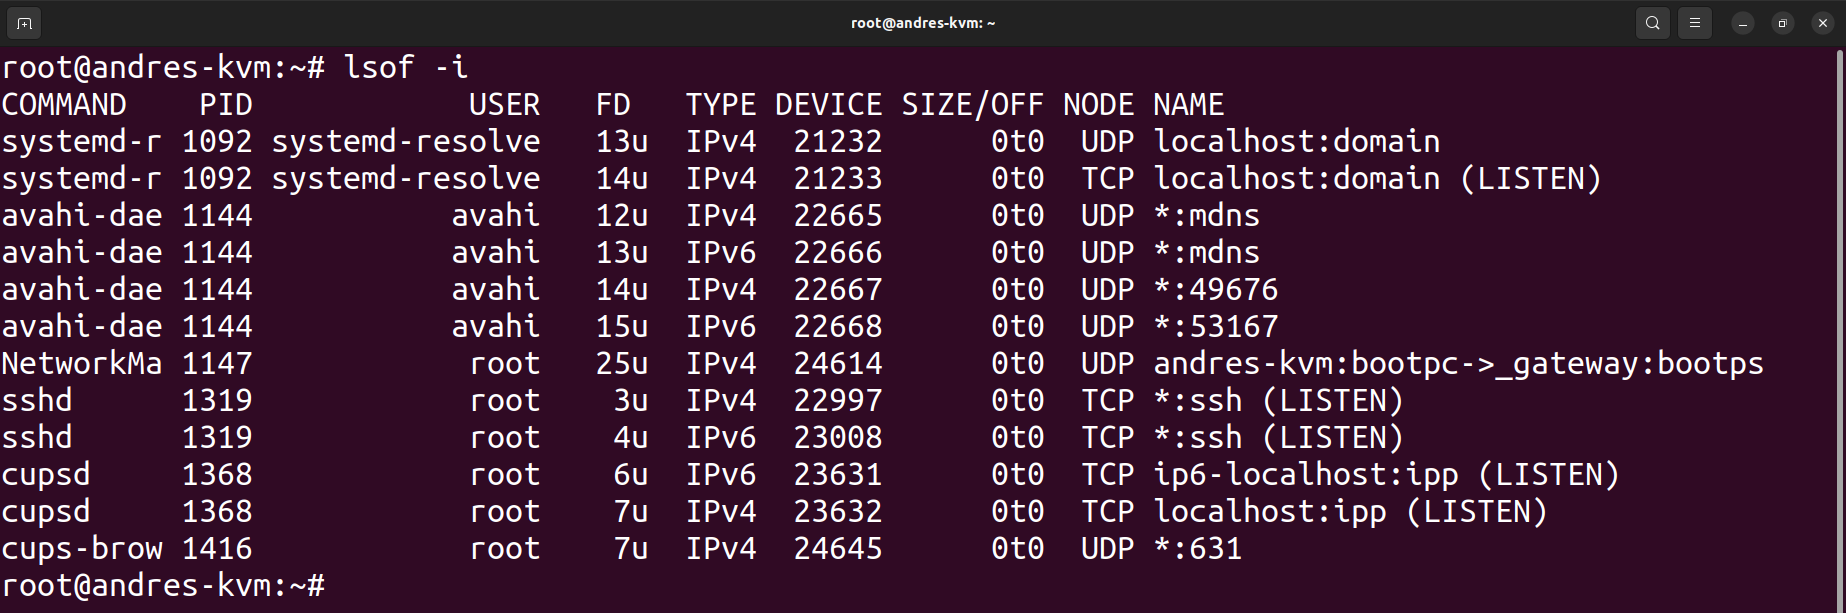
\includegraphics[width=\textwidth]{imagenes/lsofi.png}
\end{figure}

\bigskip

La orden ofrece 9 columnas con los siguientes significados:

\begin{itemize}
    \item \textbf{COMMAND: }Nombre del comando asociado al proceso/archivo.
    \item \textbf{PID: }Process IDentificator (identificador de proceso).
    \item \textbf{USER: }UID del usuario al que pertenece el proceso/archivo.
    \item \textbf{FD: }Descriptor de fichero.
    \item \textbf{TYPE: }Tipo de archivo asociado al mismo (GDIR, GREG, ...) o indica el tipo de conexión (en capa de red) (IPv4, IPv6, X.25, etc.).
    \item \textbf{DEVICE: }Número de dispositivo.
    \item \textbf{SIZE/OFF: }Tamaño del archivo.
    \item \textbf{NODE: }Número de nodo/inodo de un fichero o el protocolo en capa de transporte (TCP, UDP, ...).
    \item \textbf{NAME: }Punto de montaje y sistema de archivos que usa el archivo abierto. También puede significar la dirección local o remota de internet o de un socket.
\end{itemize}

\bigskip

A continuación explicaré dos procesos de la salida del comando anterior:

\addcontentsline{toc}{subsubsection}{sshd}
\subsubsection*{sshd}
\begin{itemize}
    \item \textbf{COMMAND: }sshd
    \item \textbf{PID: }1319
    \item \textbf{USER: }root
    \item \textbf{FD: }3u/4u (FD 3 y 4. La letra ``u'' indica acceso de lectura y escritura)
    \item \textbf{TYPE: }IPv4/IPv6 (está a la espera de recibir algo en las dos versiones del protocolo IP.)
    \item \textbf{DEVICE: }22997/23008
    \item \textbf{SIZE/OFF: }0t0 (Offset, el segundo ``0'' indica que no hay offset)
    \item \textbf{NODE: }TCP (usan este protocolo de transporte porque asegura que se reciben los paquetes mediante ACK).
    \item \textbf{NAME: }*:ssh (LISTEN) (El asterisco indica que espera de cualquier IP, en el puerto ssh (configurable, por defecto el 22)).
\end{itemize}

\addcontentsline{toc}{subsubsection}{avahi-daemon}
\subsubsection*{avahi-daemon}
\begin{itemize}
    \item \textbf{COMMAND: }avahi-dae (avahi-daemon)
    \item \textbf{PID: }1144
    \item \textbf{USER: }avahi
    \item \textbf{FD: }14u (FD 14. La letra ``u'' indica acceso de lectura y escritura)
    \item \textbf{TYPE: }IPv6
    \item \textbf{DEVICE: }22668
    \item \textbf{SIZE/OFF: }0t0 (Offset, el segundo ``0'' indica que no hay offset)
    \item \textbf{NODE: }UDP
    \item \textbf{NAME: }*:53167 (Cualquier IP en el puerto 53167).
\end{itemize}


\addcontentsline{toc}{subsection}{Apartado B}
\subsection*{Apartado B}
Leyendo el manual, hace falta usar el switch \verb|-i|, como en el apartado anterior, y añadiendo que busque las conexiones con el servicio ``ssh''. Por tanto, el comando quedaría así: \verb|lsof -i :ssh|.

\begin{figure}[H]
    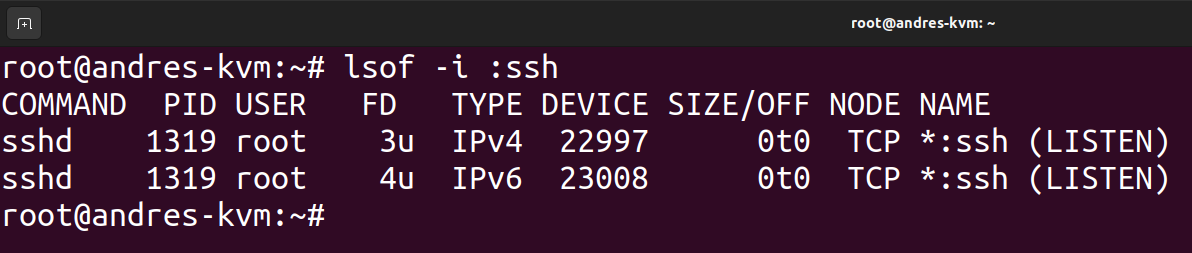
\includegraphics[width=\textwidth]{imagenes/lsofisshlisten.png}
\end{figure}

Ahora mismo no hay nadie conectado, solo están los ``daemons'' a la escucha de peticiones de conexión. Si ahora me conecto desde otra máquina virtual a la de Ubuntu, la salida es la siguiente:

\begin{figure}[H]
    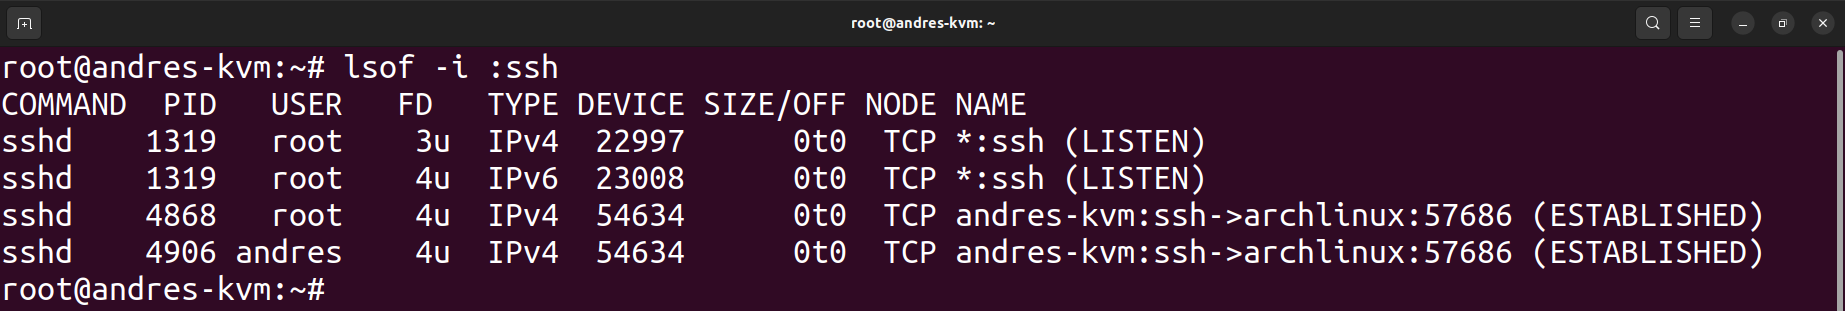
\includegraphics[width=\textwidth]{imagenes/lsofissharch.png}
\end{figure}


Aparecen dos líneas nuevas y en el apartado \verb|NAME| se ve que la conexión es entre el usuario ``andres-kvm'' (Ubuntu) usando el servicio ``ssh'' (en mi caso es el puerto 22)  y el usuario ``archlinux'' en el puerto 57686, que es un puerto que se asigna aleatoriamente para enviar información (escuchar) a ``archlinux''.

\newpage

Con la orden \verb|lsof -c sshd| se puede ver los archivos que tiene abiertos SSH:

\begin{figure}[H]
    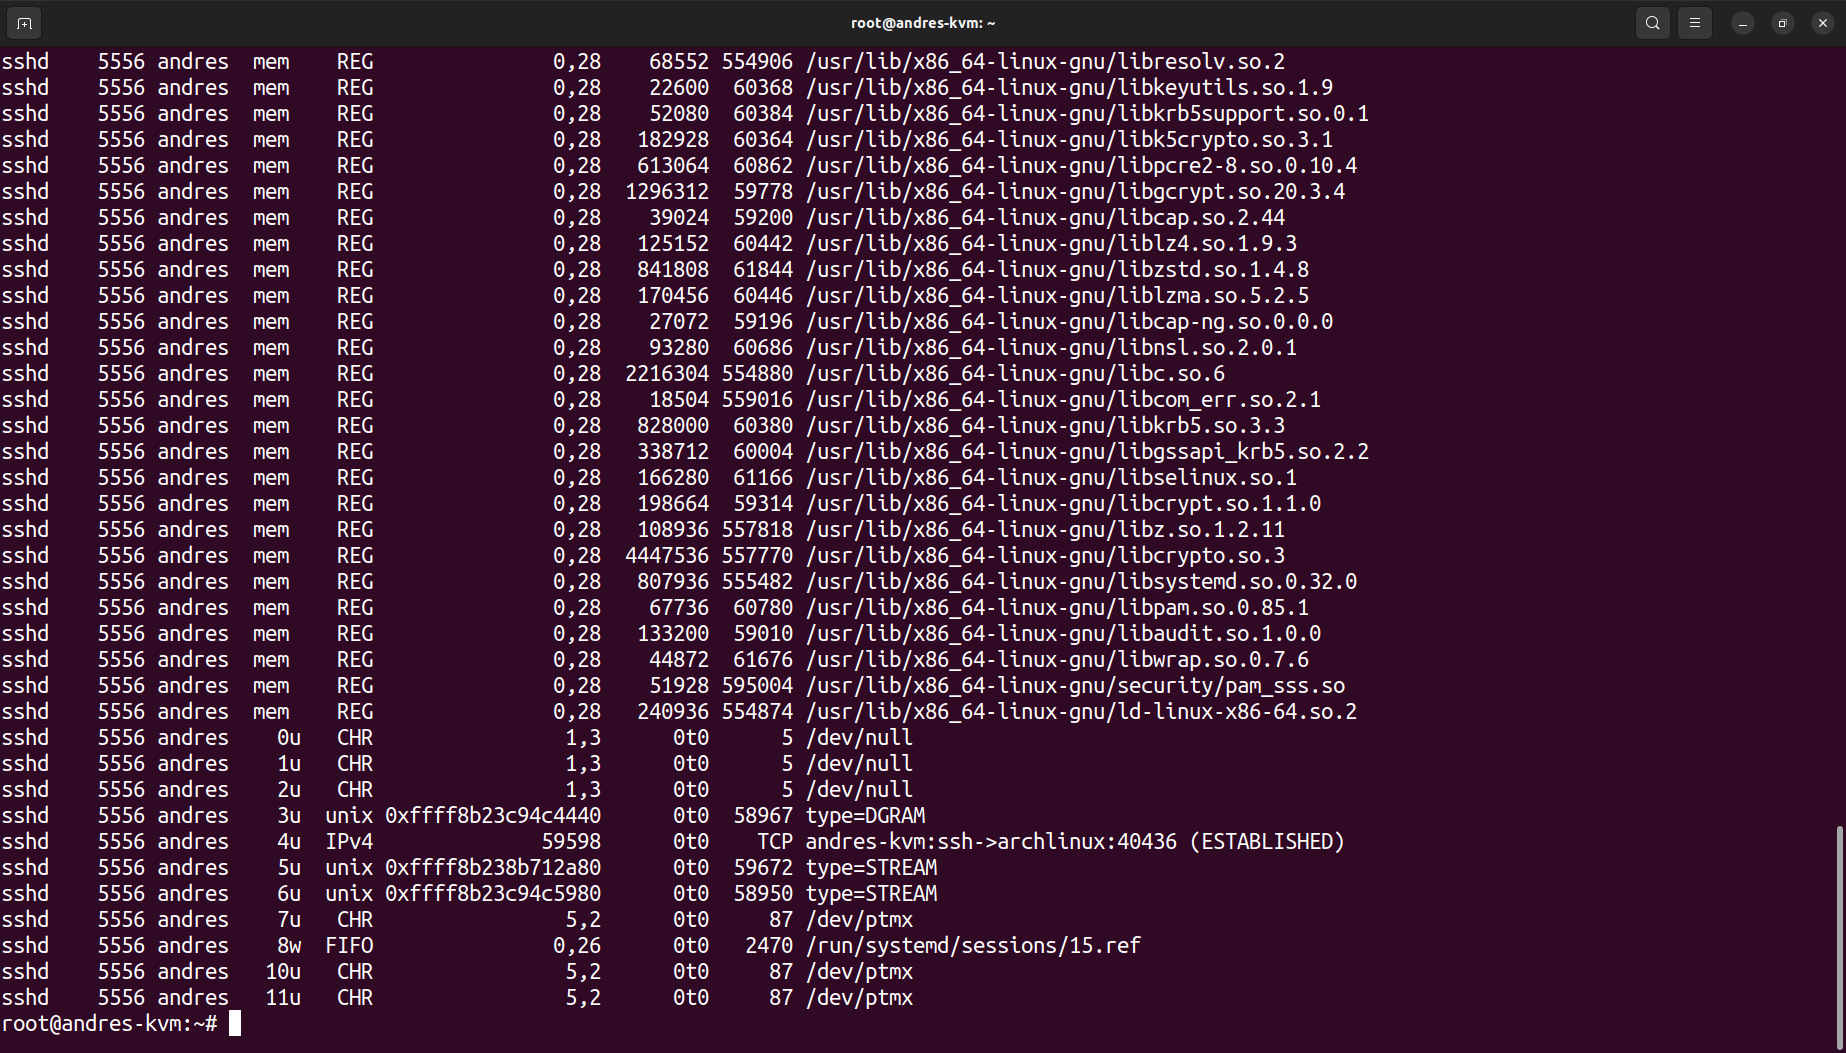
\includegraphics[width=\textwidth]{imagenes/lsofcsshd.png}
\end{figure}

Como se puede ver, aparece el usuario conectado y con el mismo PID aparecen todos los archivos abiertos por \verb|sshd|

\bigskip

\addcontentsline{toc}{subsection}{Apartado C}
\subsection*{Apartado C}
Para mostrar los archivos que usa un proceso concreto, es necesario referenciarlo con su PID. Para ello es necesario usar el siguiente comando: \verb|lsof -p PID|.

\begin{figure}[H]
    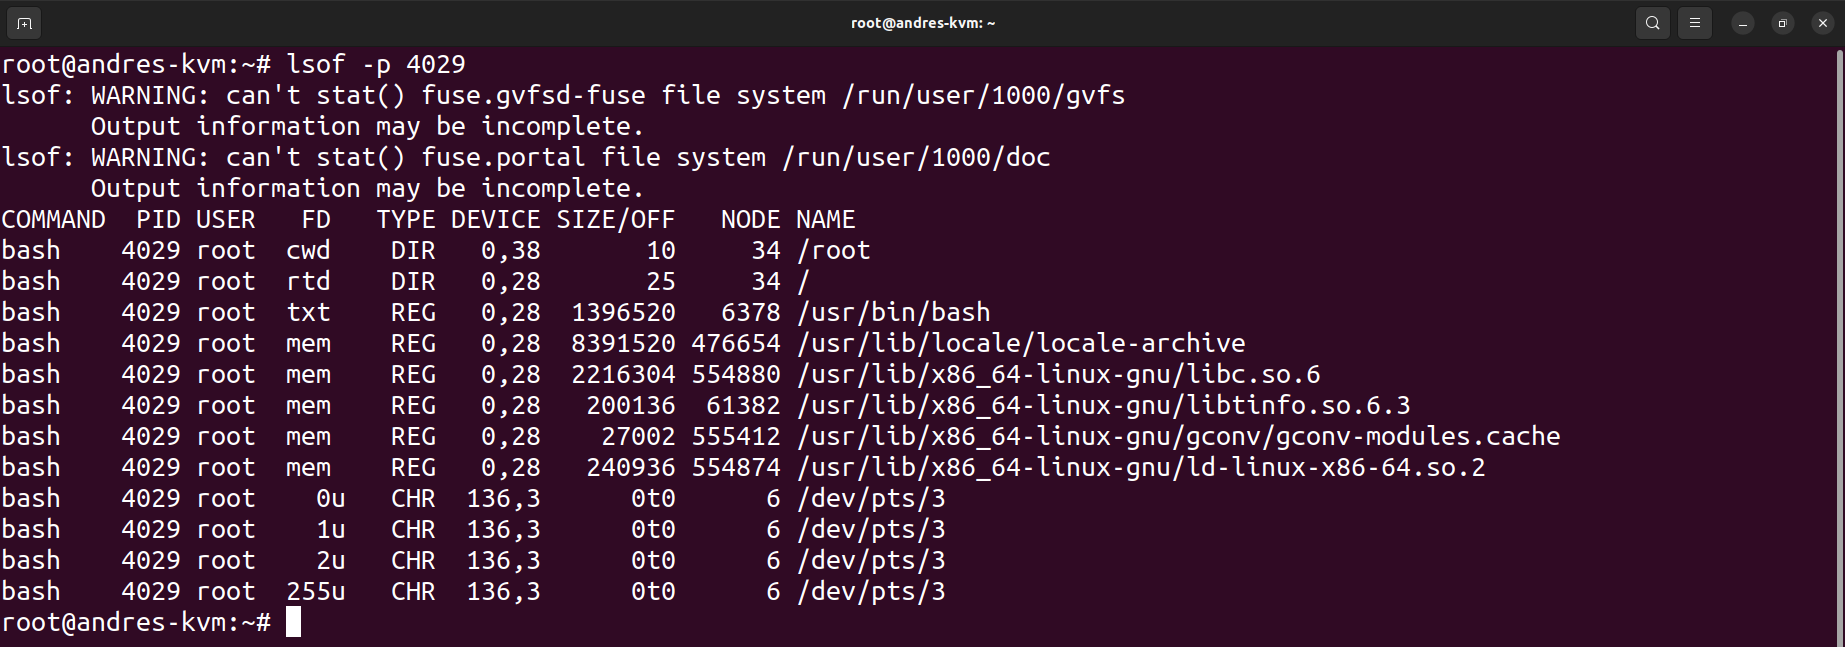
\includegraphics[width=\textwidth]{imagenes/lsofp.png}
\end{figure} 

\newpage

Y ahora para ver los archivos que está usando un usuario concreto, se debe usar el switch \verb|-u|: \verb|lsof -u usuario|

\begin{figure}[H]
    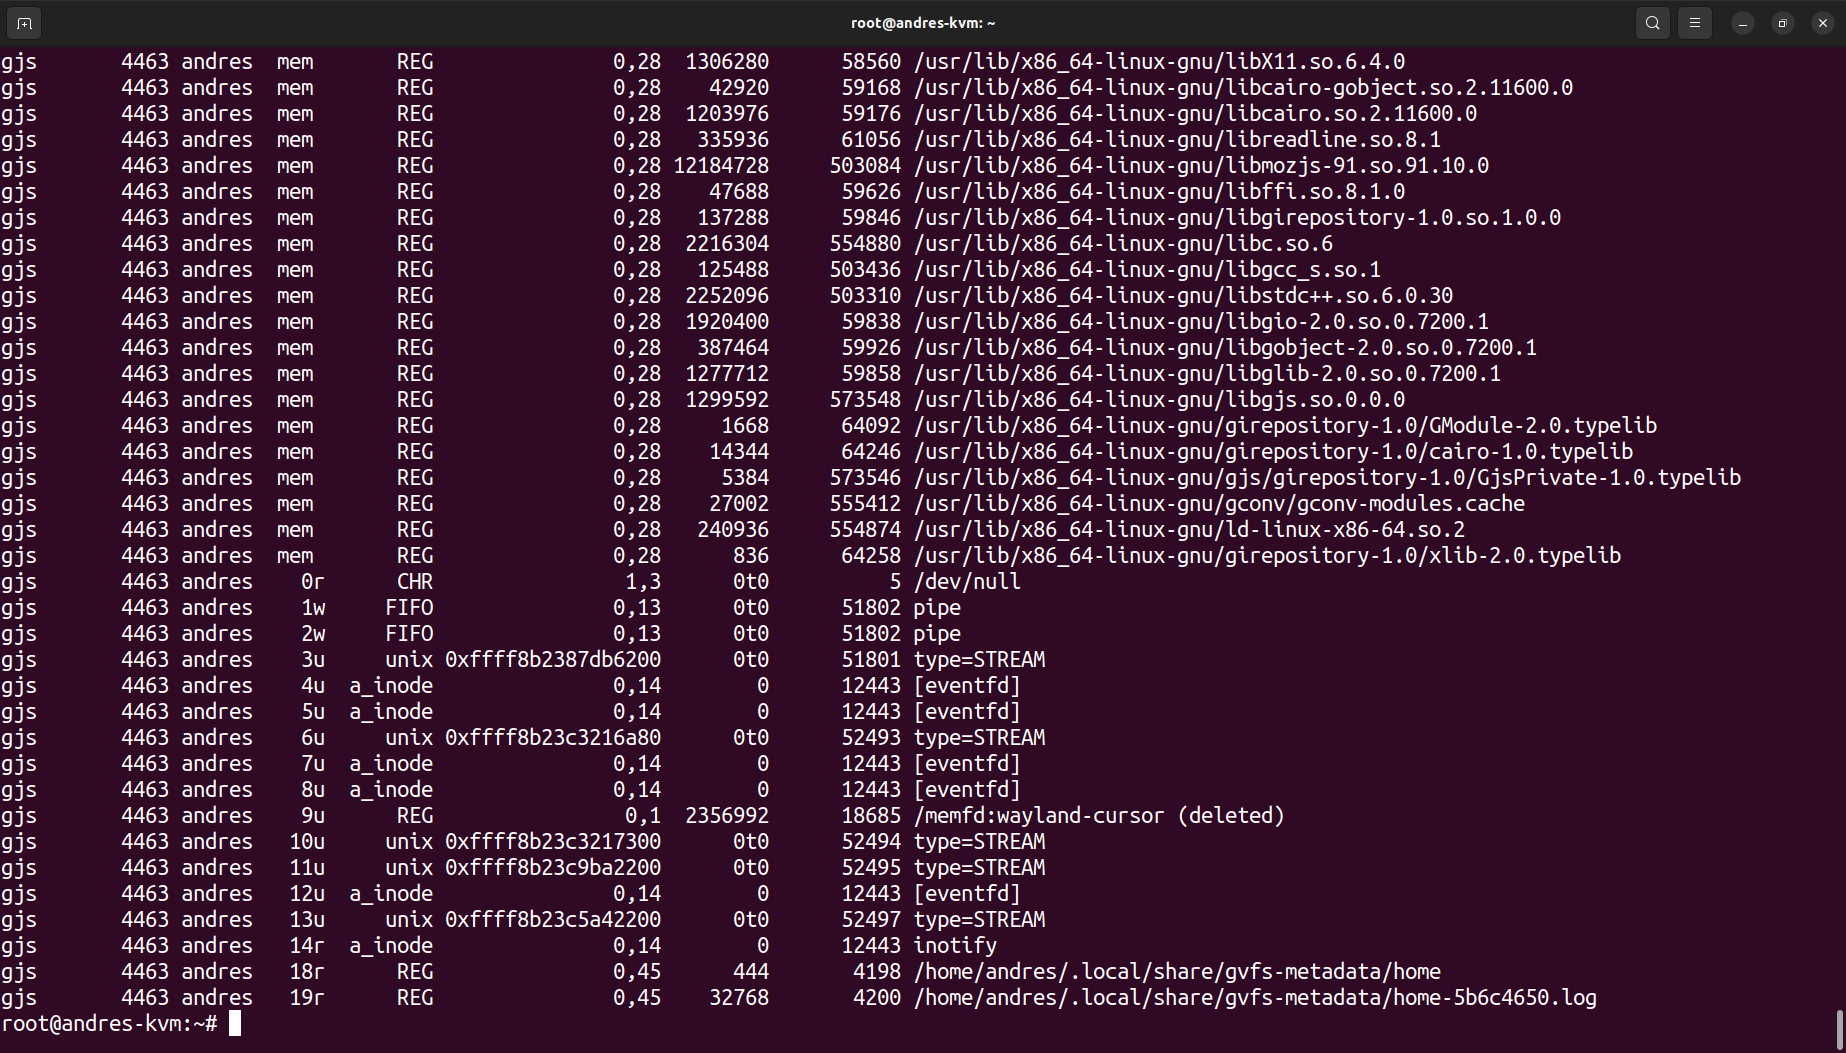
\includegraphics[width=\textwidth]{imagenes/lsofuandres.png}
    \caption{Salida de ``lsof -u andres'', se puede ver que en la tercera columna solo aparece ese usuario.}
\end{figure}

\bigskip

Por último, para obtener los archivos que tiene abiertos un proceso \textbf{Y} un usuario, es necesario usar el switch adicional \verb|-a|. Esto es debido a que por defecto solo busca, en caso de haber varios switches, utilizando un criterio \textbf{OR}. Comando: \verb|lsof -u usuario -p PID -a|

\begin{figure}[H]
    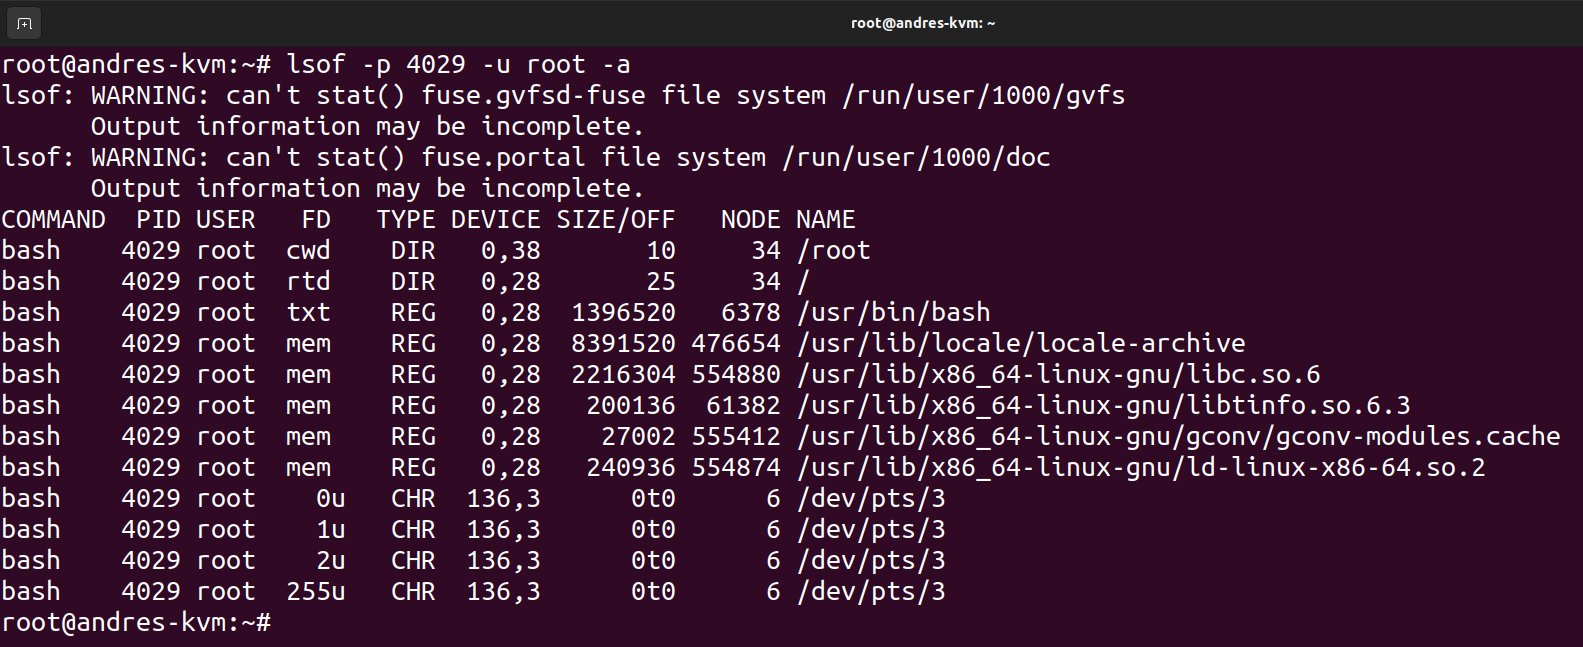
\includegraphics[width=\textwidth]{imagenes/lsofand.png}
    \caption{Archivos abiertos por el PID 4029 \textbf{Y} el usuario root}
\end{figure}


\newpage

\addcontentsline{toc}{section}{Ejercicio 2}
\section*{Ejercicio 2}
\addcontentsline{toc}{subsection}{Apartado A}
\subsection*{Apartado A}
Para ver que vulnerabilidades hay en el sistema es necesario instalar el paquete \verb|lynis| junto al comando \verb|lynis audit system|.

\begin{figure}[H]
    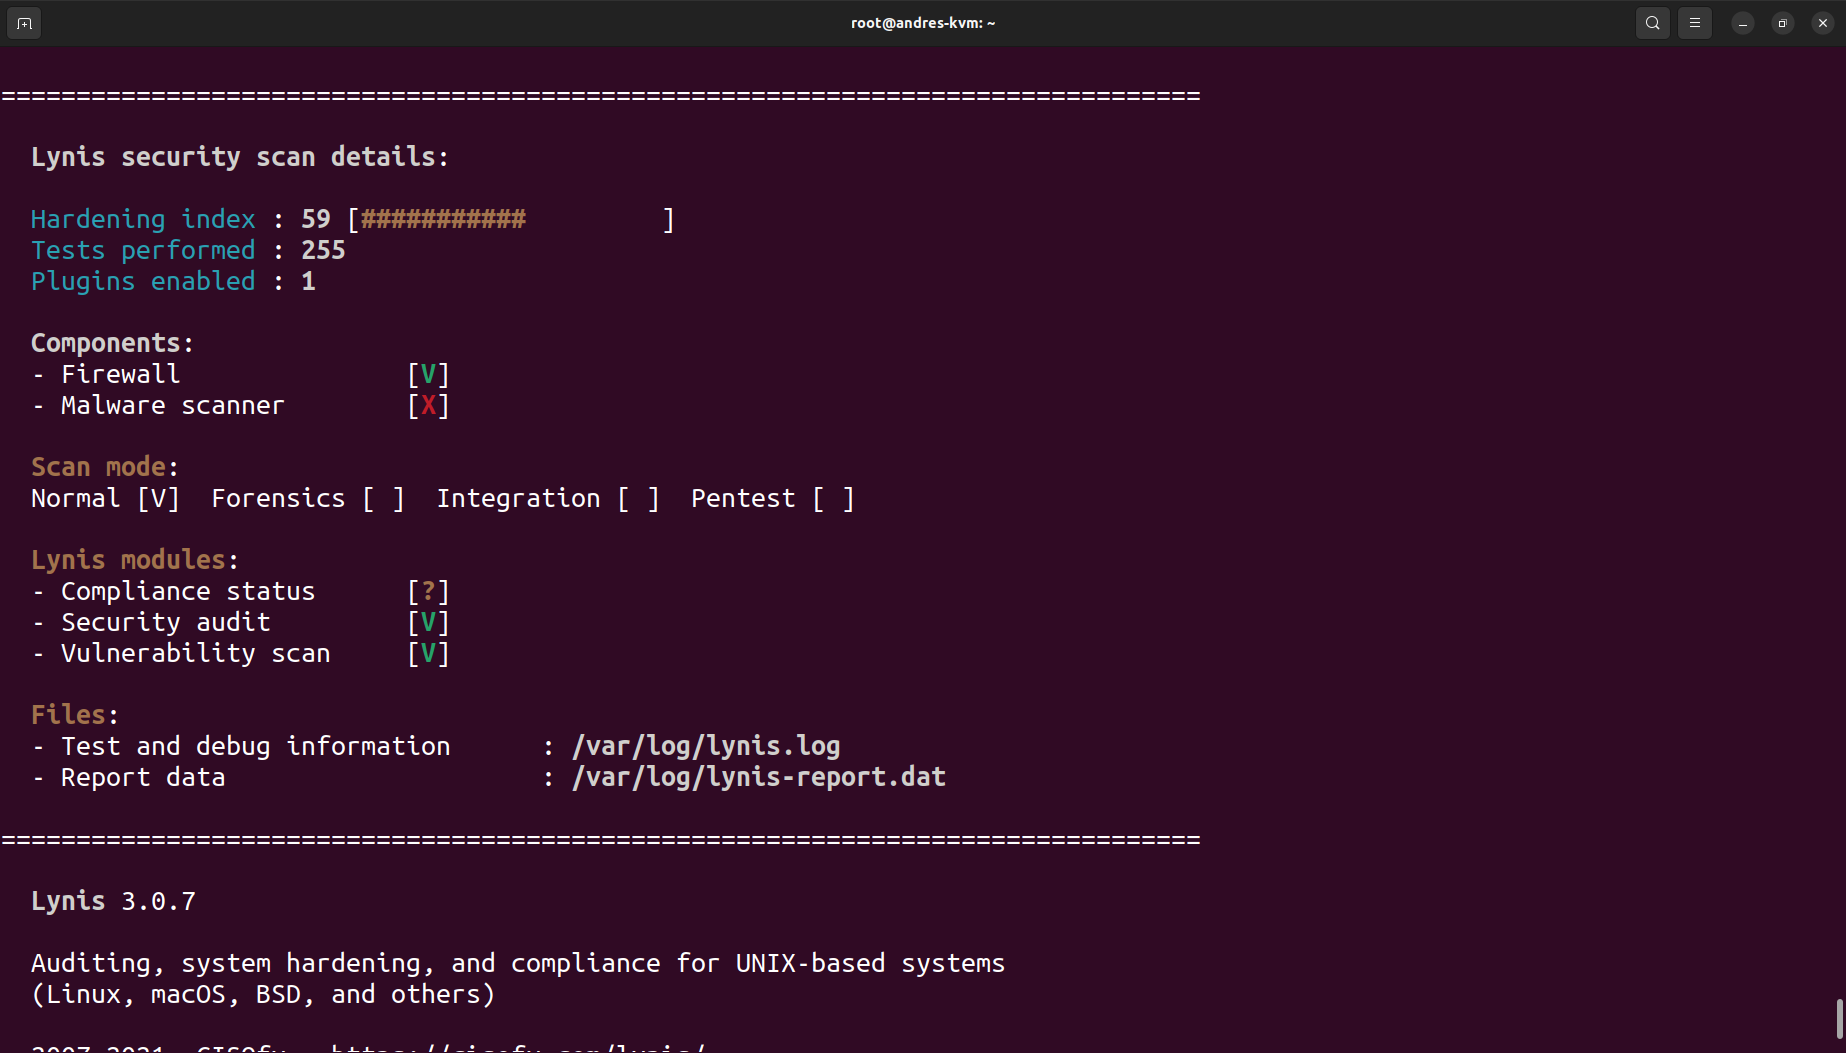
\includegraphics[width=\textwidth]{imagenes/lynisresults1.png}
\end{figure}

\bigskip

Y las posibles vulnerabilidades son las siguientes:

\begin{figure}[H]
    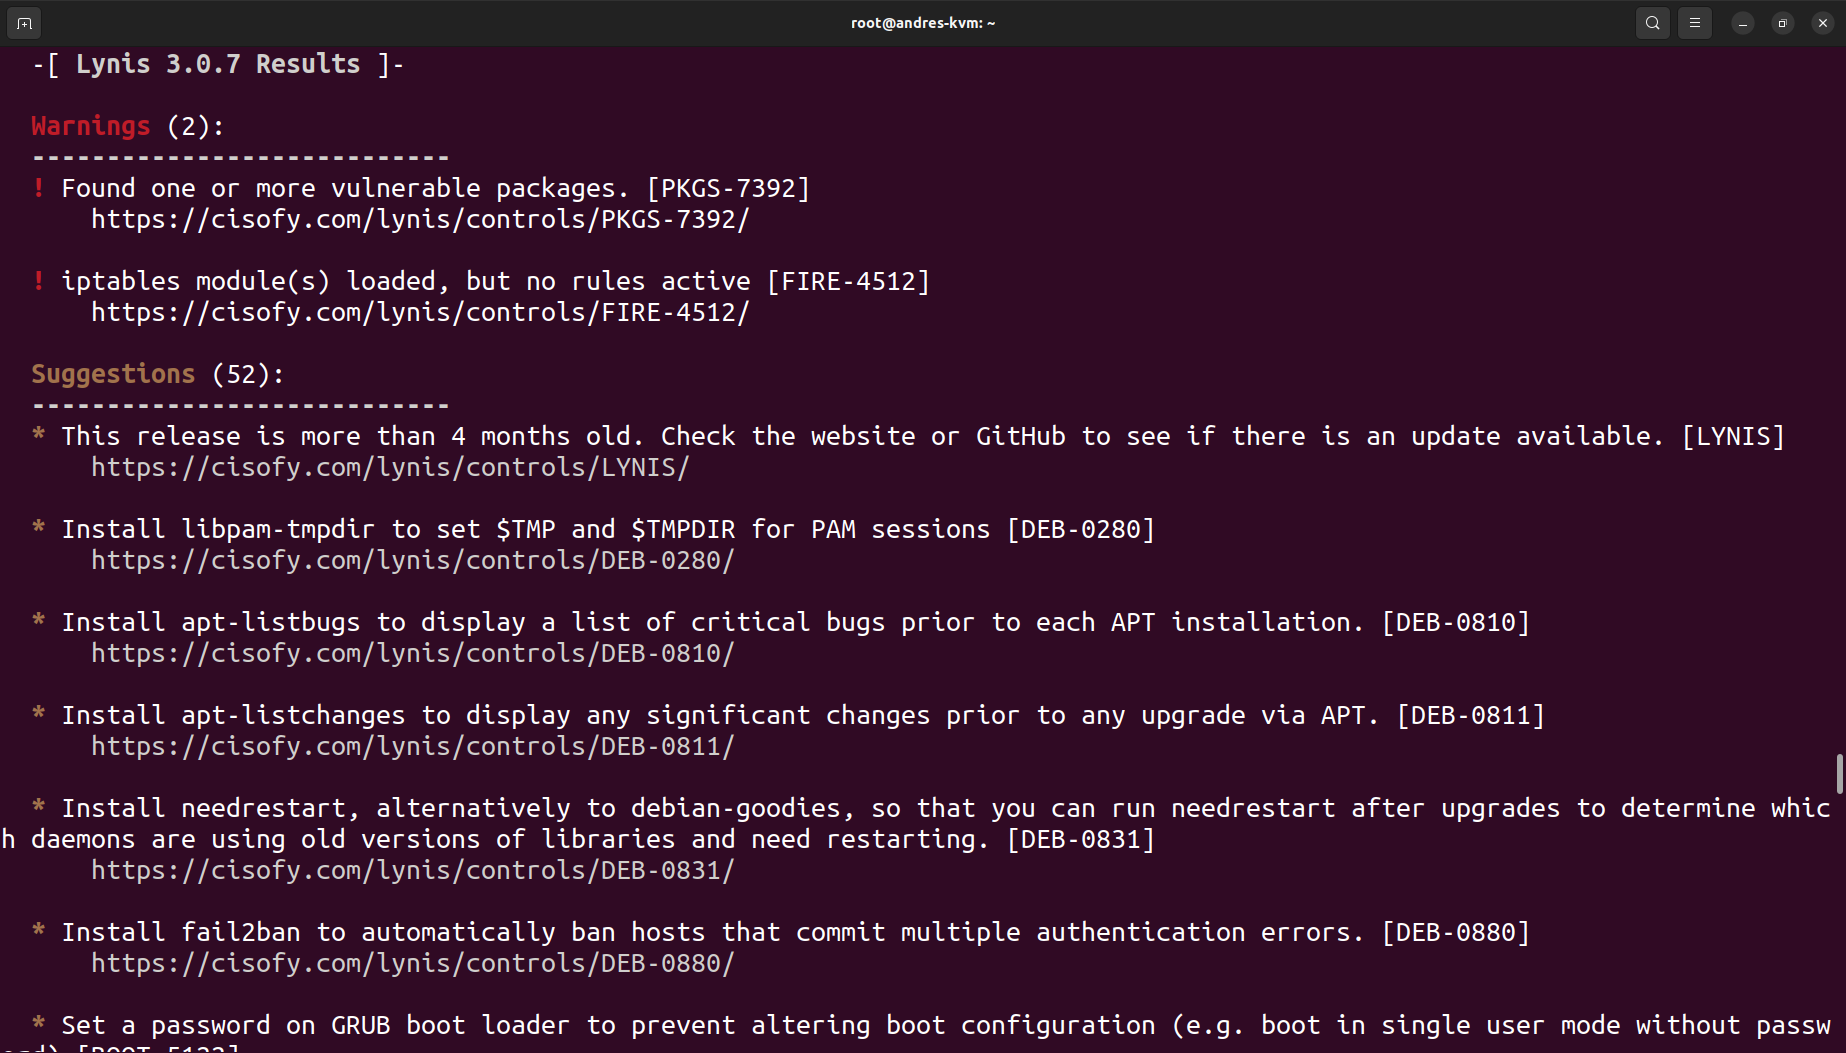
\includegraphics[width=\textwidth]{imagenes/lyniswarnings1.png}
\end{figure}

\newpage

Como se puede ver, solo hay dos avisos. Suponiendo que es una máquina para desarrollar aplicaciones, voy a listar los grados de severidad:

\begin{itemize}
    \item \textbf{Found one or more vulnerable packages. [PKGS-7392]} $\rightarrow$ Severidad: \textbf{Alta}. Puede llegar a ser muy peligroso, ya que pueden ser vulnerabilidades que potencialmente le otorguen acceso root al sistema. 
    
    \textbf{Solución: }Para solucionarlo, es necesario actualizar todos los paquetes del sistema con la orden (en Ubuntu y en distros basadas en Debian) \verb|sudo apt upgrade|.


    \item \textbf{iptables module(s) loaded, but no rules active [FIRE-4512]} $\rightarrow$ Severidad: \textbf{Alta}. \verb|iptables| es un paquete que se utiliza principalmente junto a un firewall para permitir o bloquear cierto tráfico. Si fuera una compañía importante sin firewall, podría darse el caso de que alguien entrase en el sistema y obtuviese datos sin permiso, produciendo así un ``leak'' o incluso pidiendo un rescate para no publicar la información (que en este caso podrían ser aplicaciones que no se desean que se publiquen aún).
    
    \textbf{Solución: }La solución es habilitar el firewall y aplicarle las reglas que sean necesarias. En Ubuntu viene instalado por defecto \verb|ufw|, pero viene deshabilitado. Para habilitarlo hay que poner: \verb|sudo ufw enable| y con la orden \verb|sudo ufw status verbose| se pueden ver las reglas (por defecto prohíbe tráfico entrante y permite trafico saliente, prohibiendo así conexiones del tipo SSH).

    \begin{figure}[H]
        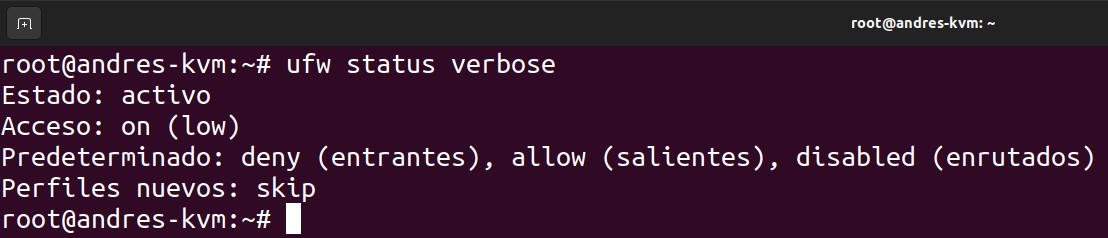
\includegraphics[width=\textwidth]{imagenes/ufwstatus.png}
    \end{figure}
\end{itemize}

\bigskip

Ahora, ejecutando de nuevo \verb|lynis audit system| aparece la siguiente puntuación:

\begin{figure}[H]
    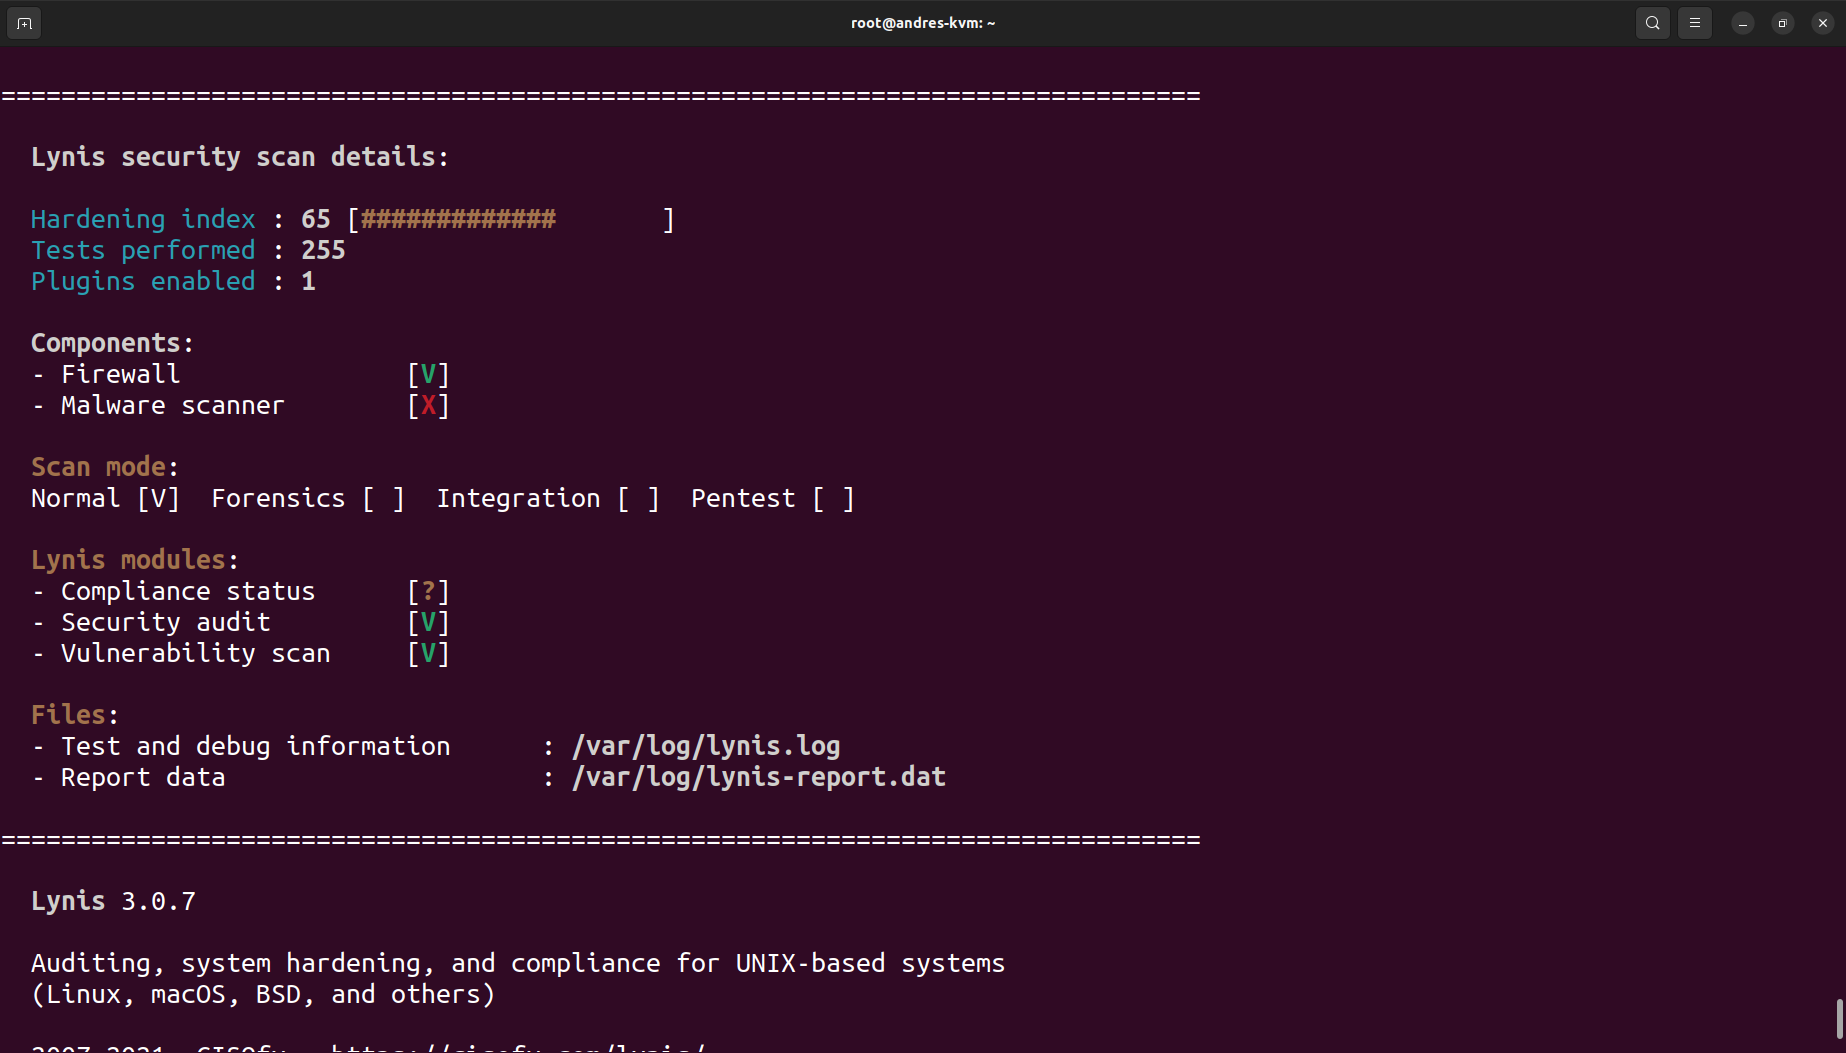
\includegraphics[width=\textwidth]{imagenes/lynisresults2.png}
\end{figure}

\newpage

Y al ver los warnings se ve que no aparece ninguno:

\begin{figure}[H]
    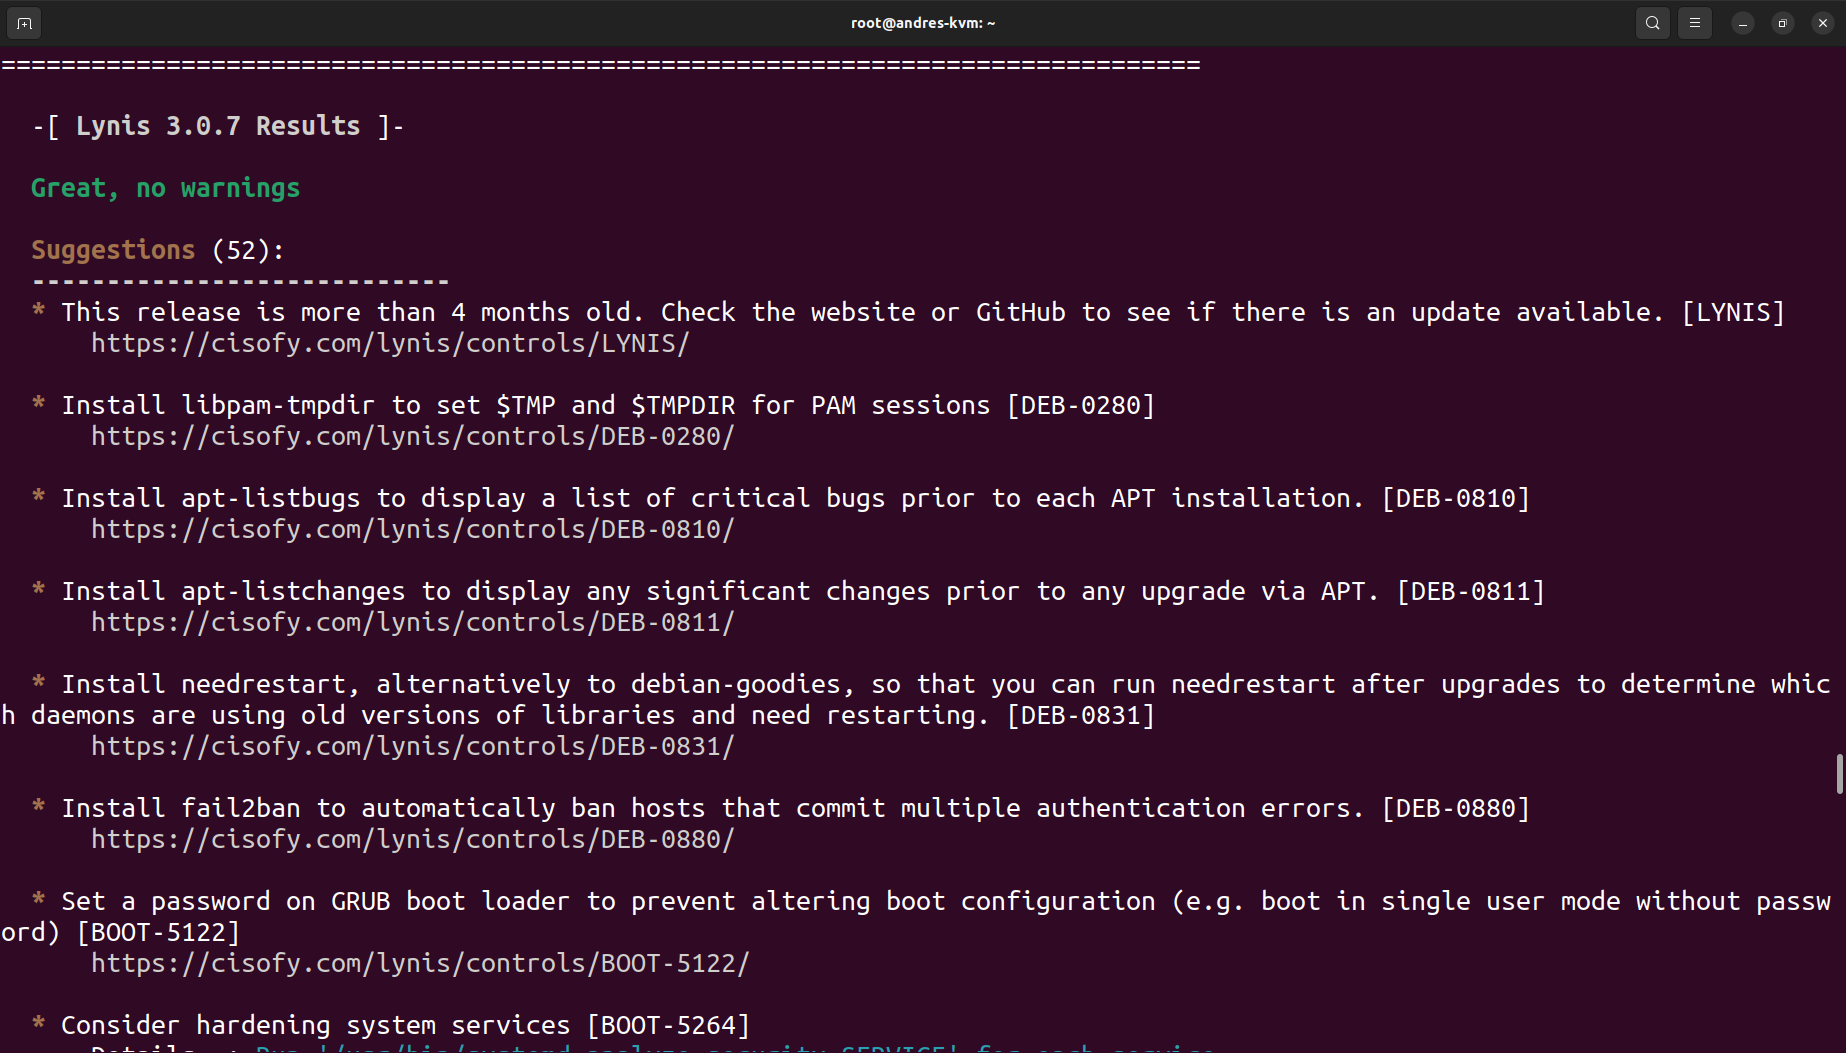
\includegraphics[width=\textwidth]{imagenes/lyniswarnings2.png}
\end{figure}

Por tanto, en cuanto a advertencias el sistema ya está ``seguro'' (nunca se puede decir con total seguridad). En cuanto a las sugerencias, las principales son para reforzar SSH y el uso de bloqueadores de IP como \verb|fail2ban|. No son fallos demasiado críticos.

\bigskip

\addcontentsline{toc}{subsection}{Apartado B}
\subsection*{Apartado B}
Lynis permite añadir nuevos tests o modificar existentes para añadirles más funcionalidad. Todo esto se realiza mediante los archivos que se encuentran en el directorio \verb|/usr/share/lynis/include|.

En este caso, para poder ver los antivirus que detecta actualmente es necesario inspeccionar el archivo \verb|/usr/share/lynis/include/tests_malware|:

\begin{figure}[H]
    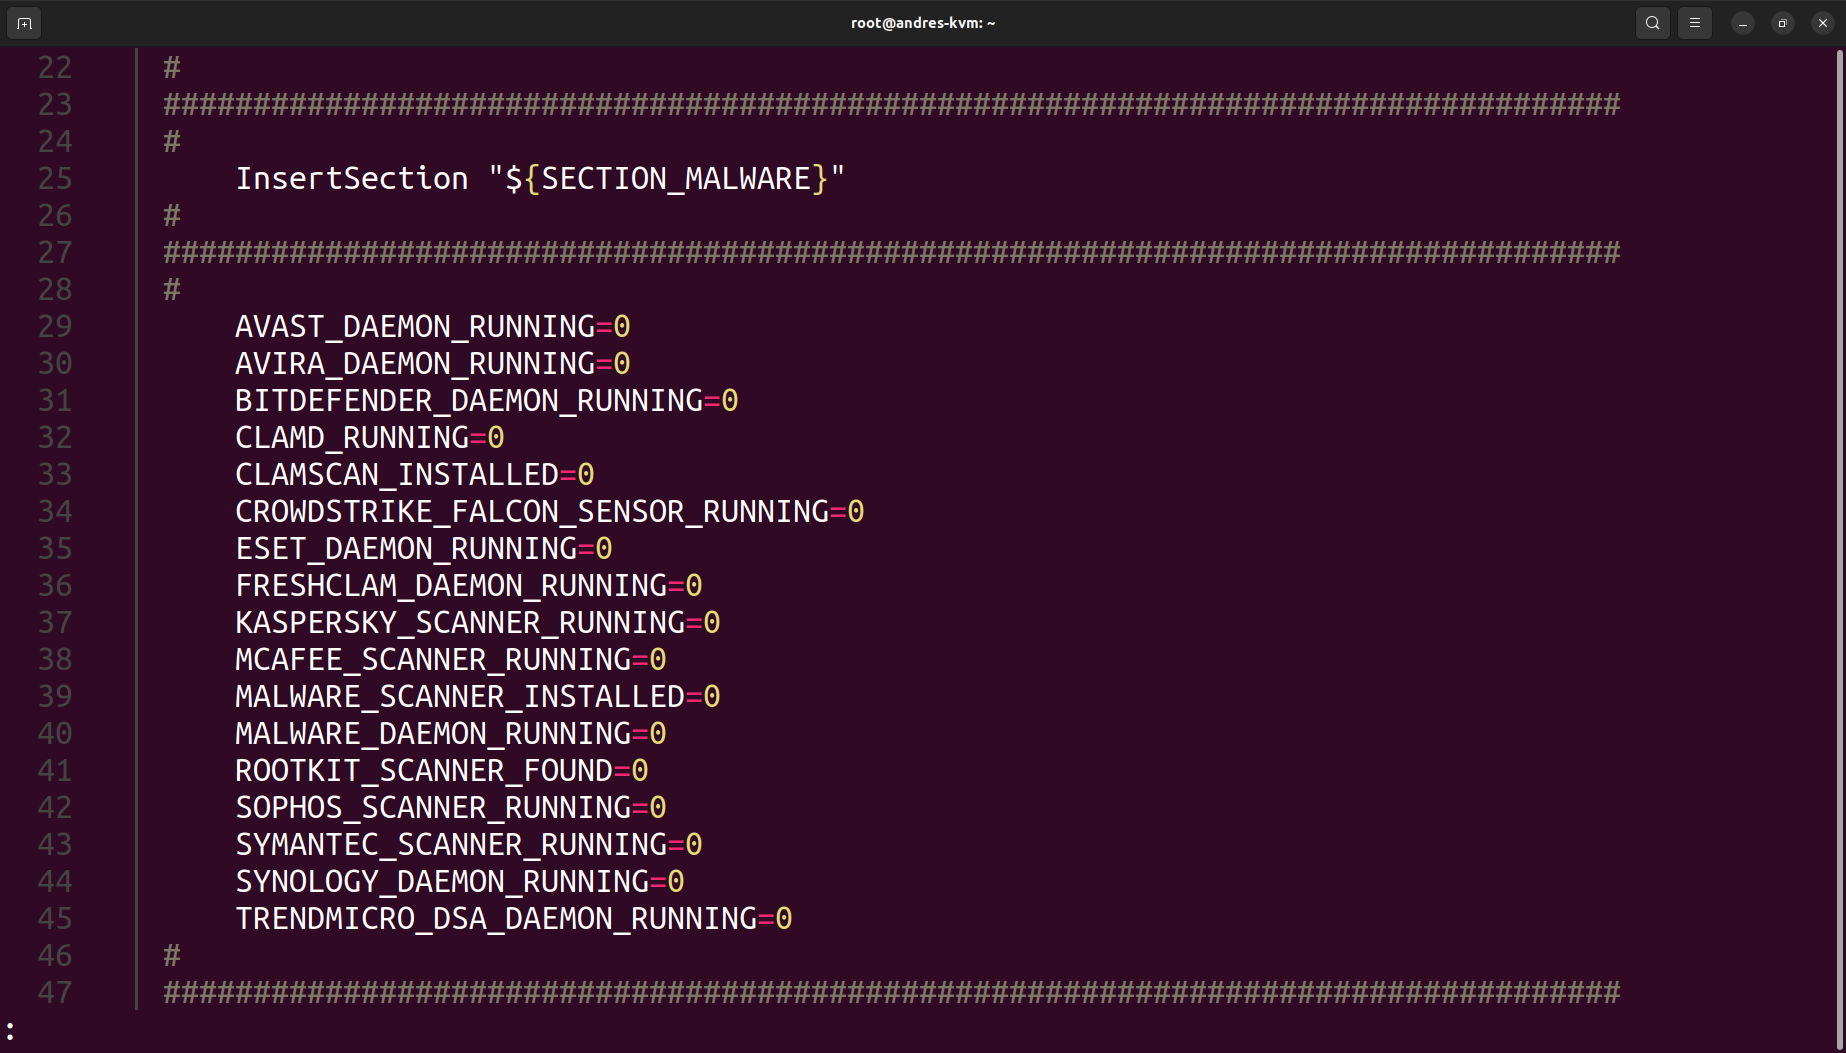
\includegraphics[width=\textwidth]{imagenes/antivirus1.png}
\end{figure}

\newpage

Como se puede ver, detecta los siguientes antivirus: 

\begin{itemize}
    \item Avast
    \item Avira
    \item Bitdefender
    \item ClamAV (clamd, clamscan y freshclam)
    \item CrowdStrike
    \item ESET
    \item Kaspersky
    \item McAfee
    \item chkrootkit
    \item rkhunter
    \item LMD
    \item CylanceSvc
    \item SophosScanD
    \item Symantec
    \item Synology Antivirus Essential
    \item Trend Micro Anti Malware for Linux
\end{itemize}

\bigskip

Ahora voy a instalar el programa \verb|unhide|, el cual no es detectado por Lynis:

\begin{figure}[H]
    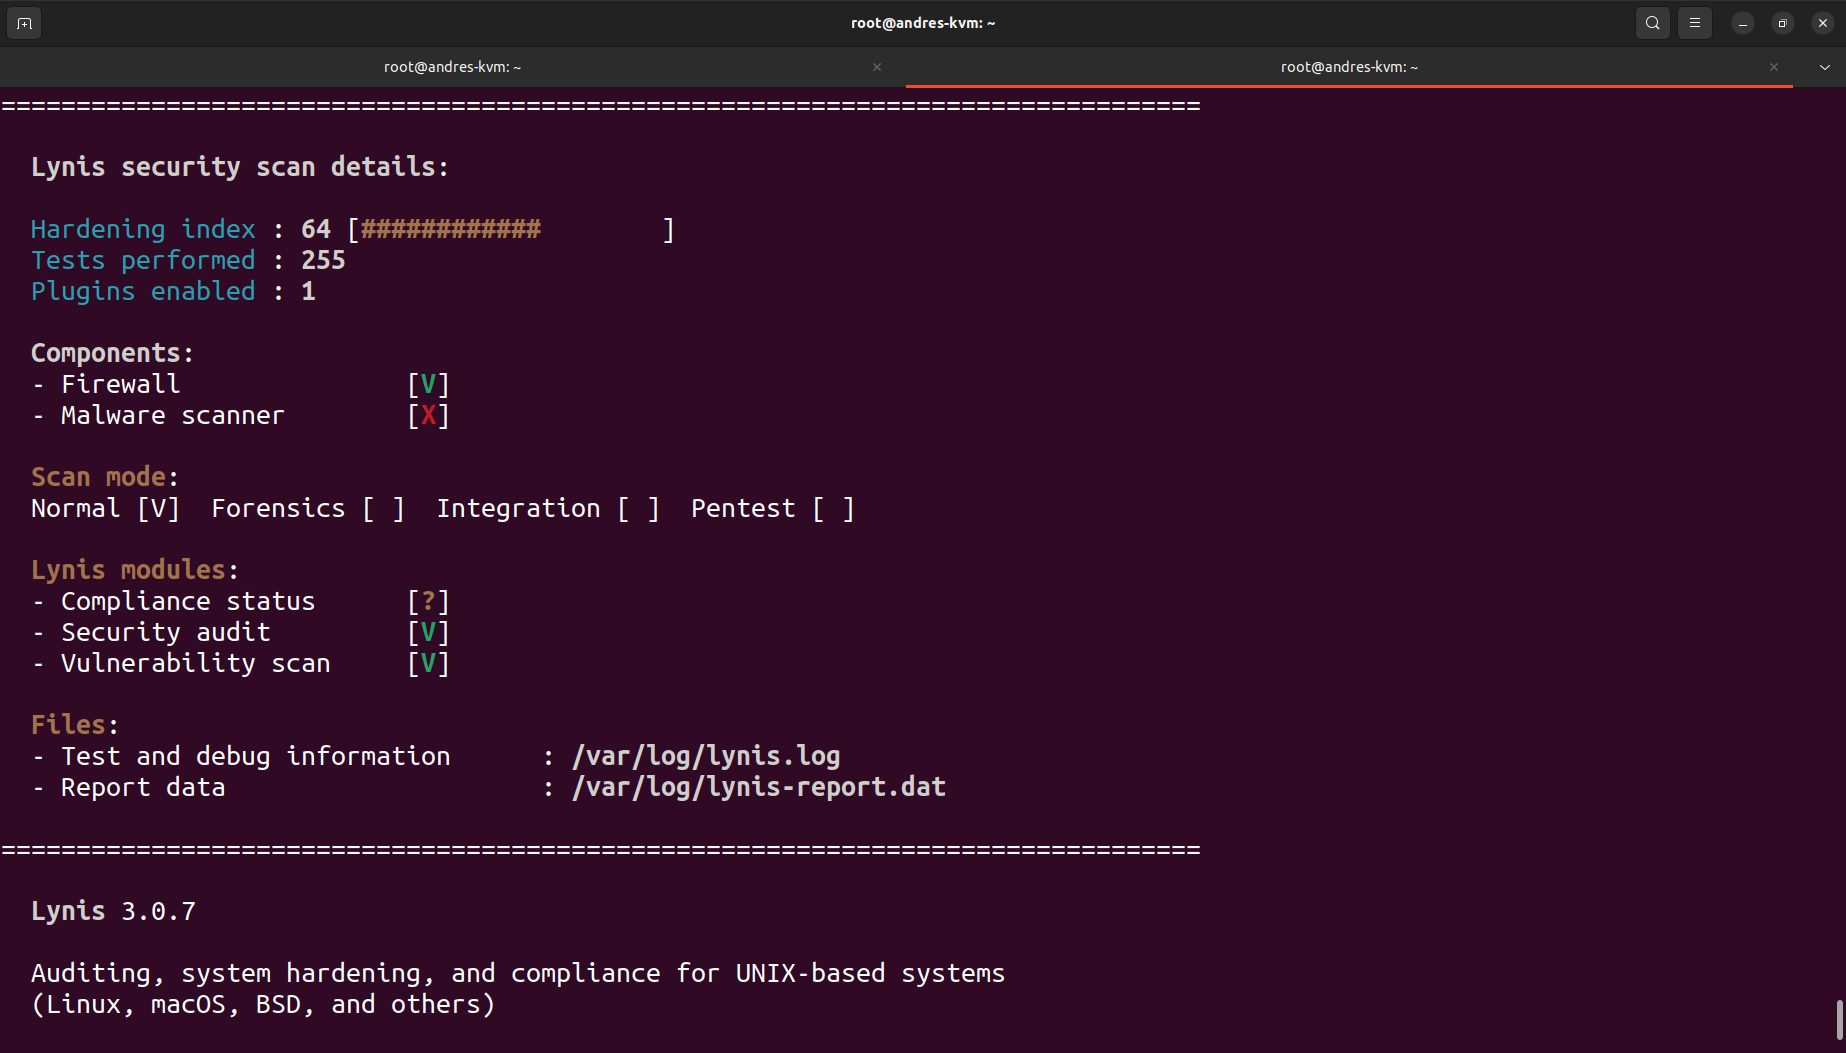
\includegraphics[width=\textwidth]{imagenes/lynisresults3unhide.png}
    \caption{Indica que no hay un antivirus, cuando realmente hay un tipo de protección (unhide).}
\end{figure}

\newpage

Ahora, modifico el archivo anterior y añado la macro:

\begin{figure}[H]
    \centering
    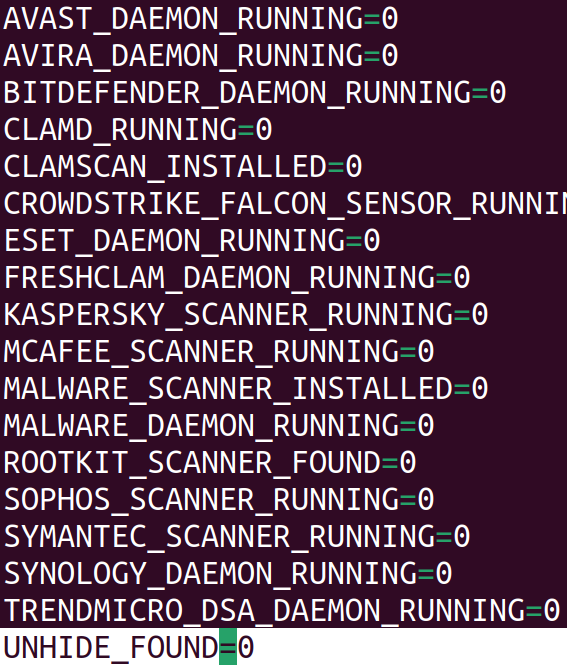
\includegraphics[width=0.5\textwidth]{imagenes/macro.png}
\end{figure}

\bigskip

Y añadimos un nuevo ``if'' en la cadena del test ``MALW-3280'':

\begin{figure}[H]
    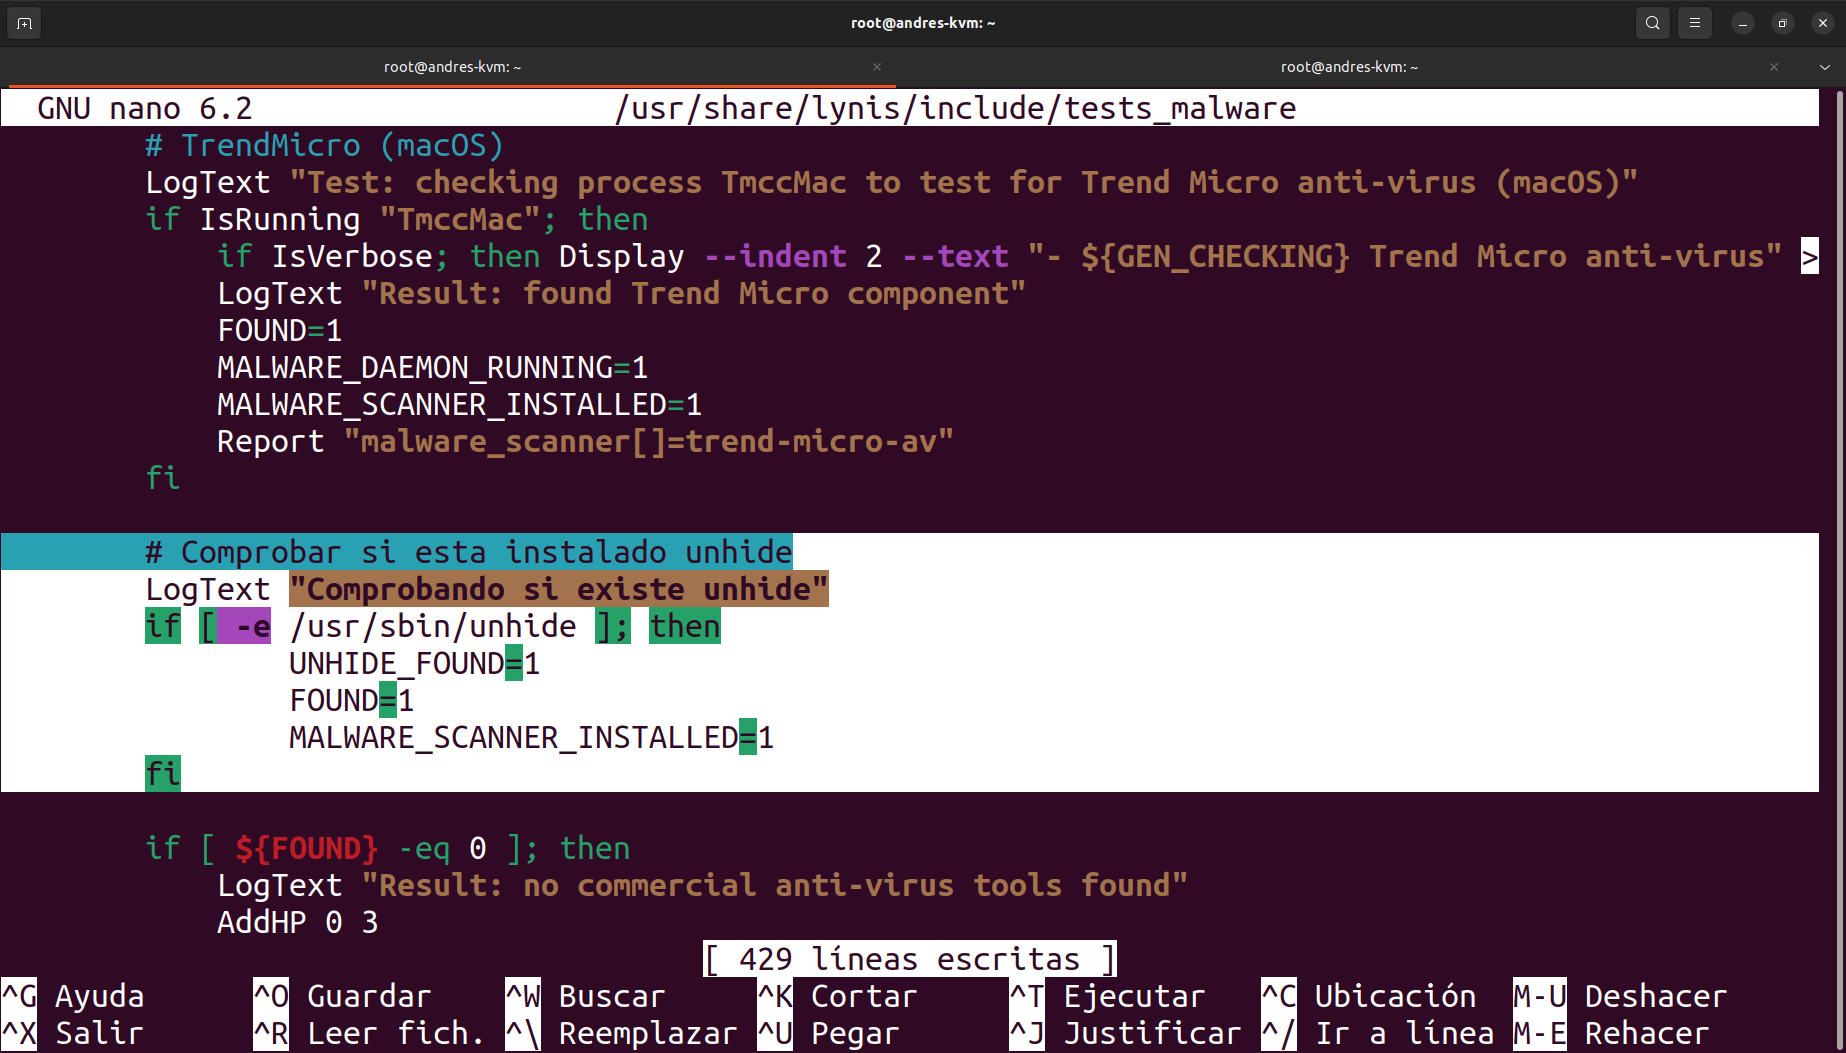
\includegraphics[width=\textwidth]{imagenes/unhidetest.png}
\end{figure}

\newpage

Ahora al pasar el test ya aparece como que existe un antivirus:

\begin{figure}[H]
    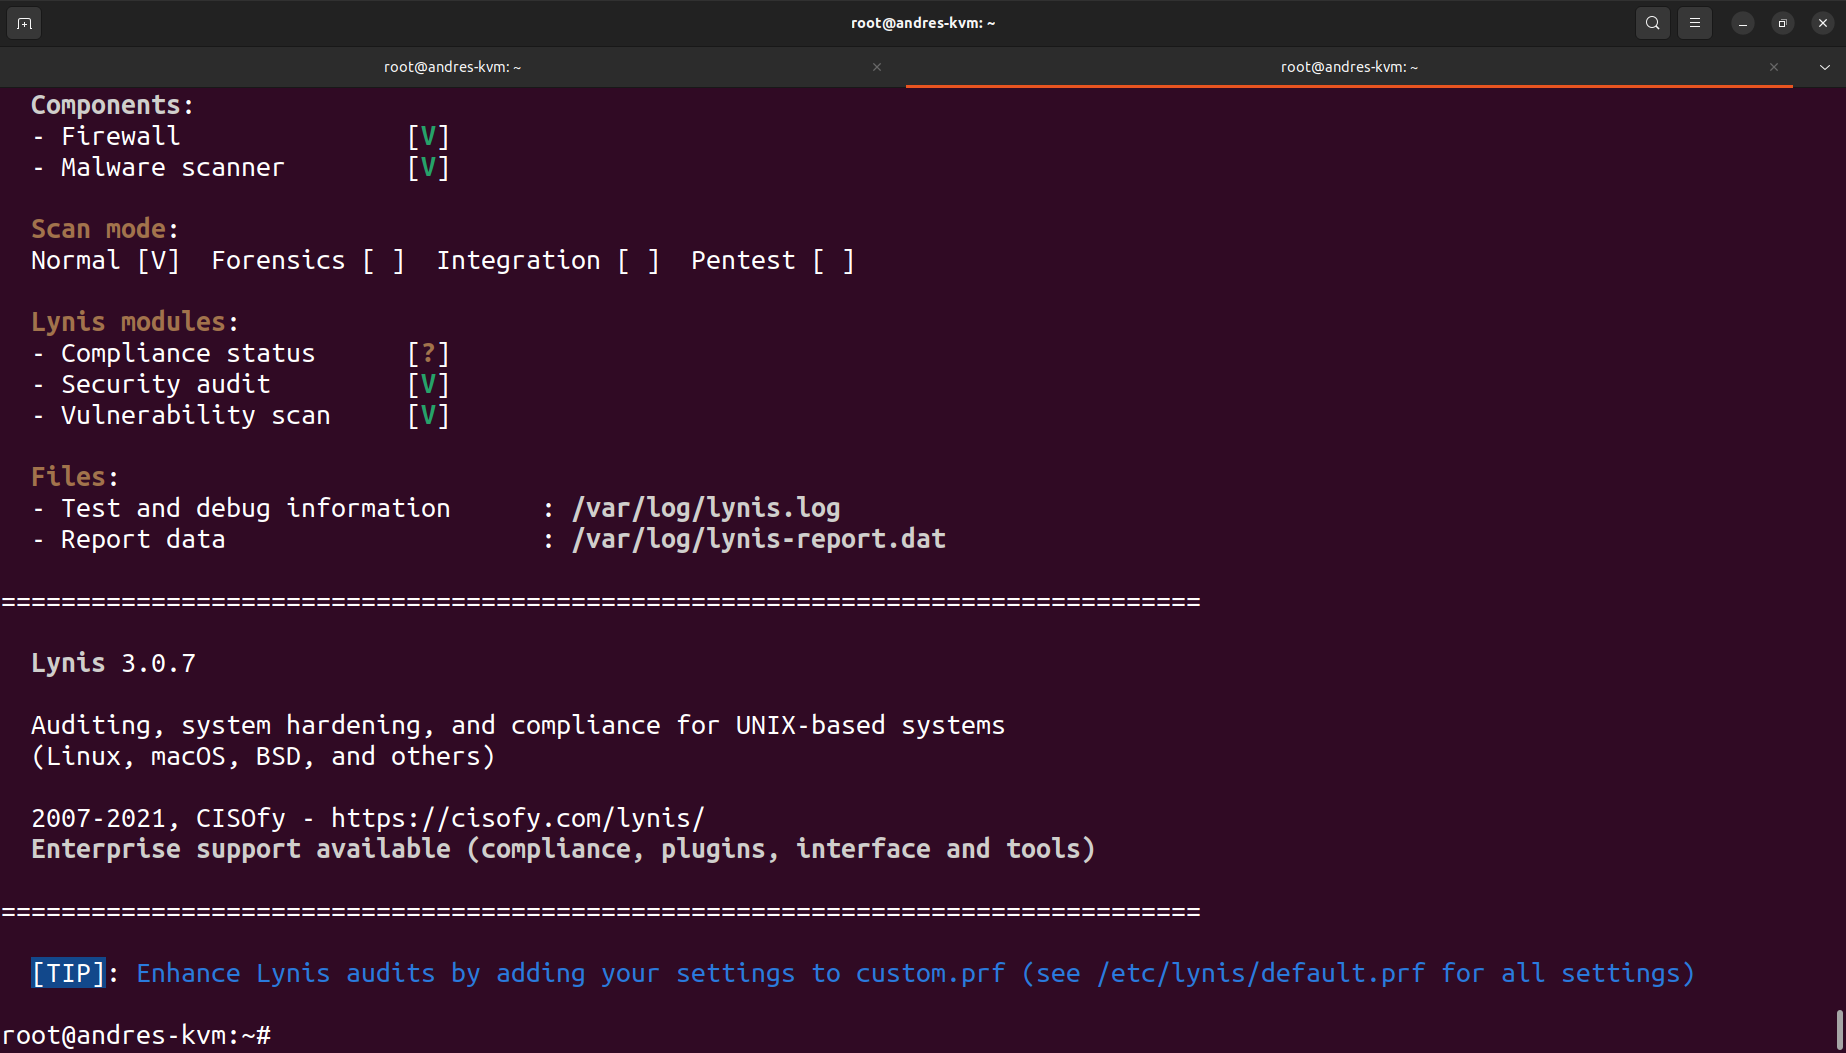
\includegraphics[width=\textwidth]{imagenes/lynisok.png}
    \caption{Se puede observar el resultado en la tercera línea.}
\end{figure}

\bigskip

Y si desinstalo \verb|unhide| aparece como que no hay ningún antivirus instalado:

\begin{figure}[H]
    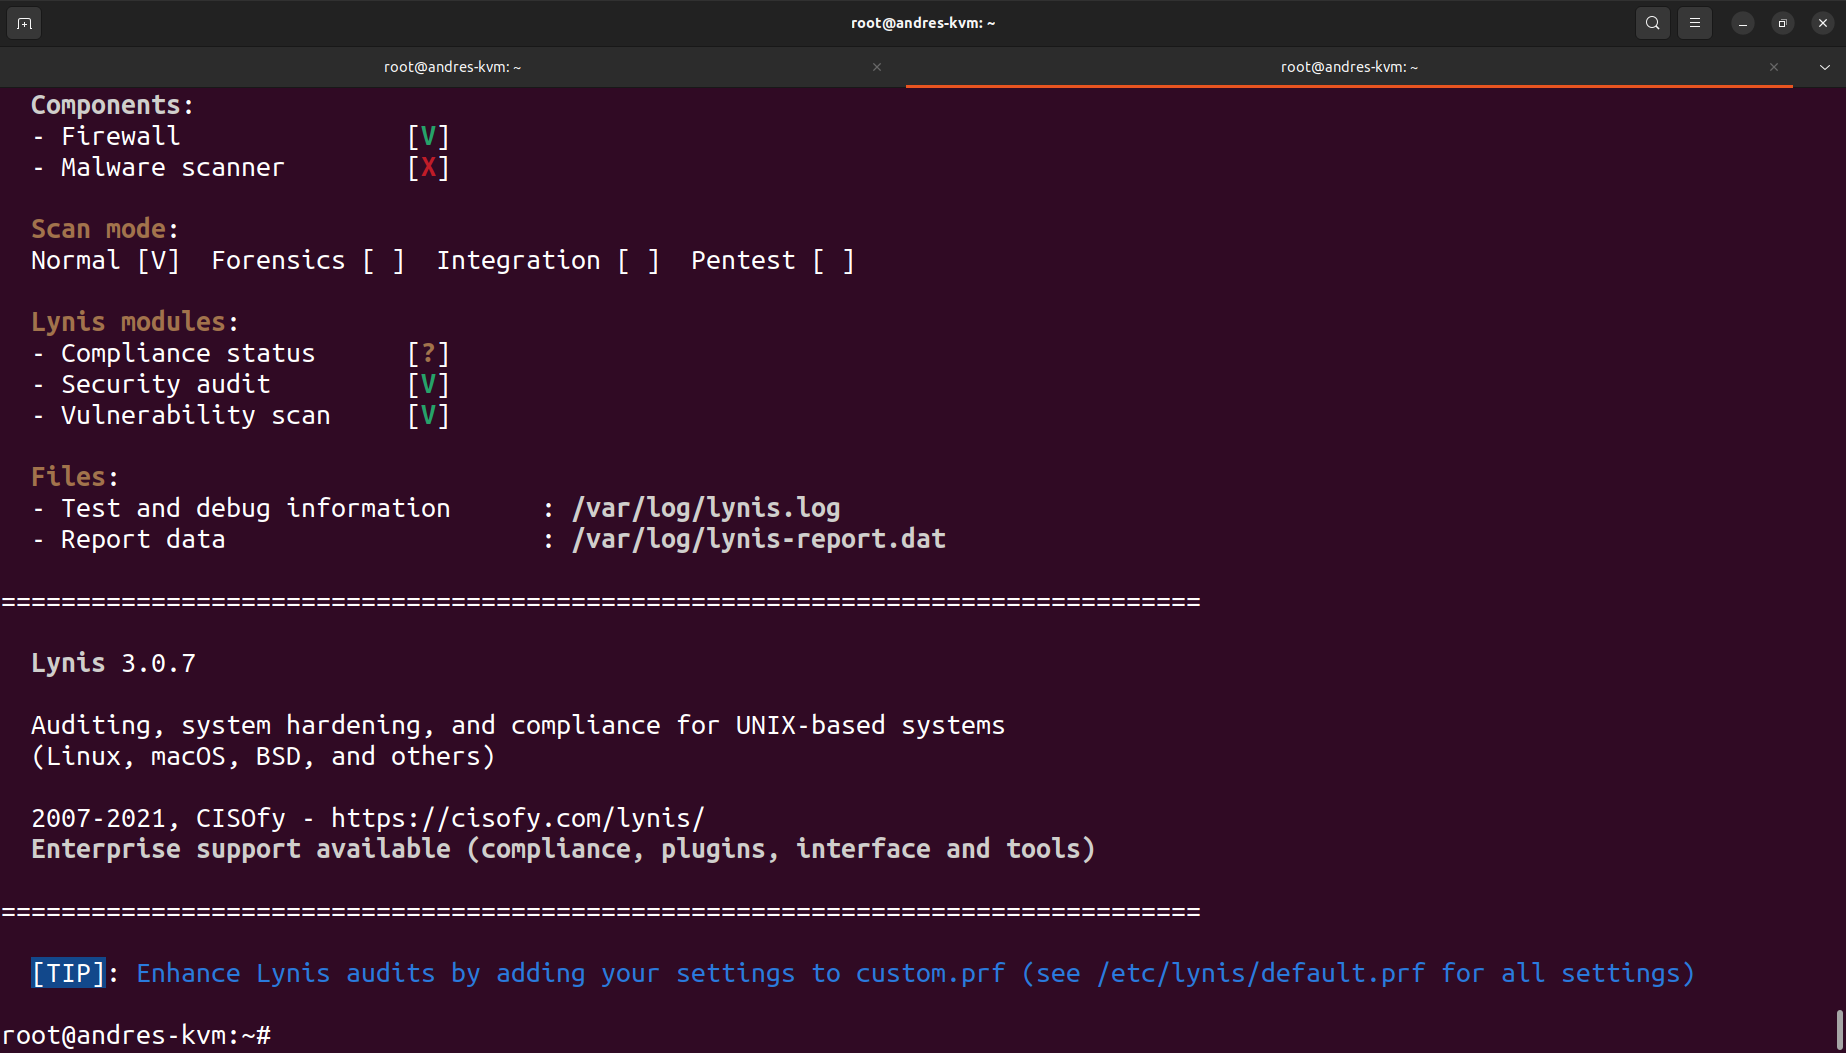
\includegraphics[width=\textwidth]{imagenes/lynisnook.png}
    \caption{Se puede observar el resultado en la tercera línea.}
\end{figure}


\newpage

\addcontentsline{toc}{section}{Ejercicio 3}
\subsection*{Ejercicio 3}

Para instalar la herramienta en Ubuntu se ejecuta la orden: \verb|sudo apt install rkhunter|.

\addcontentsline{toc}{subsection}{Apartado A}
\subsection*{Apartado A}
Para realizar el análisis es necesario ejecutar el comando: \verb|sudo rkhunter --check|

\begin{figure}[H]
    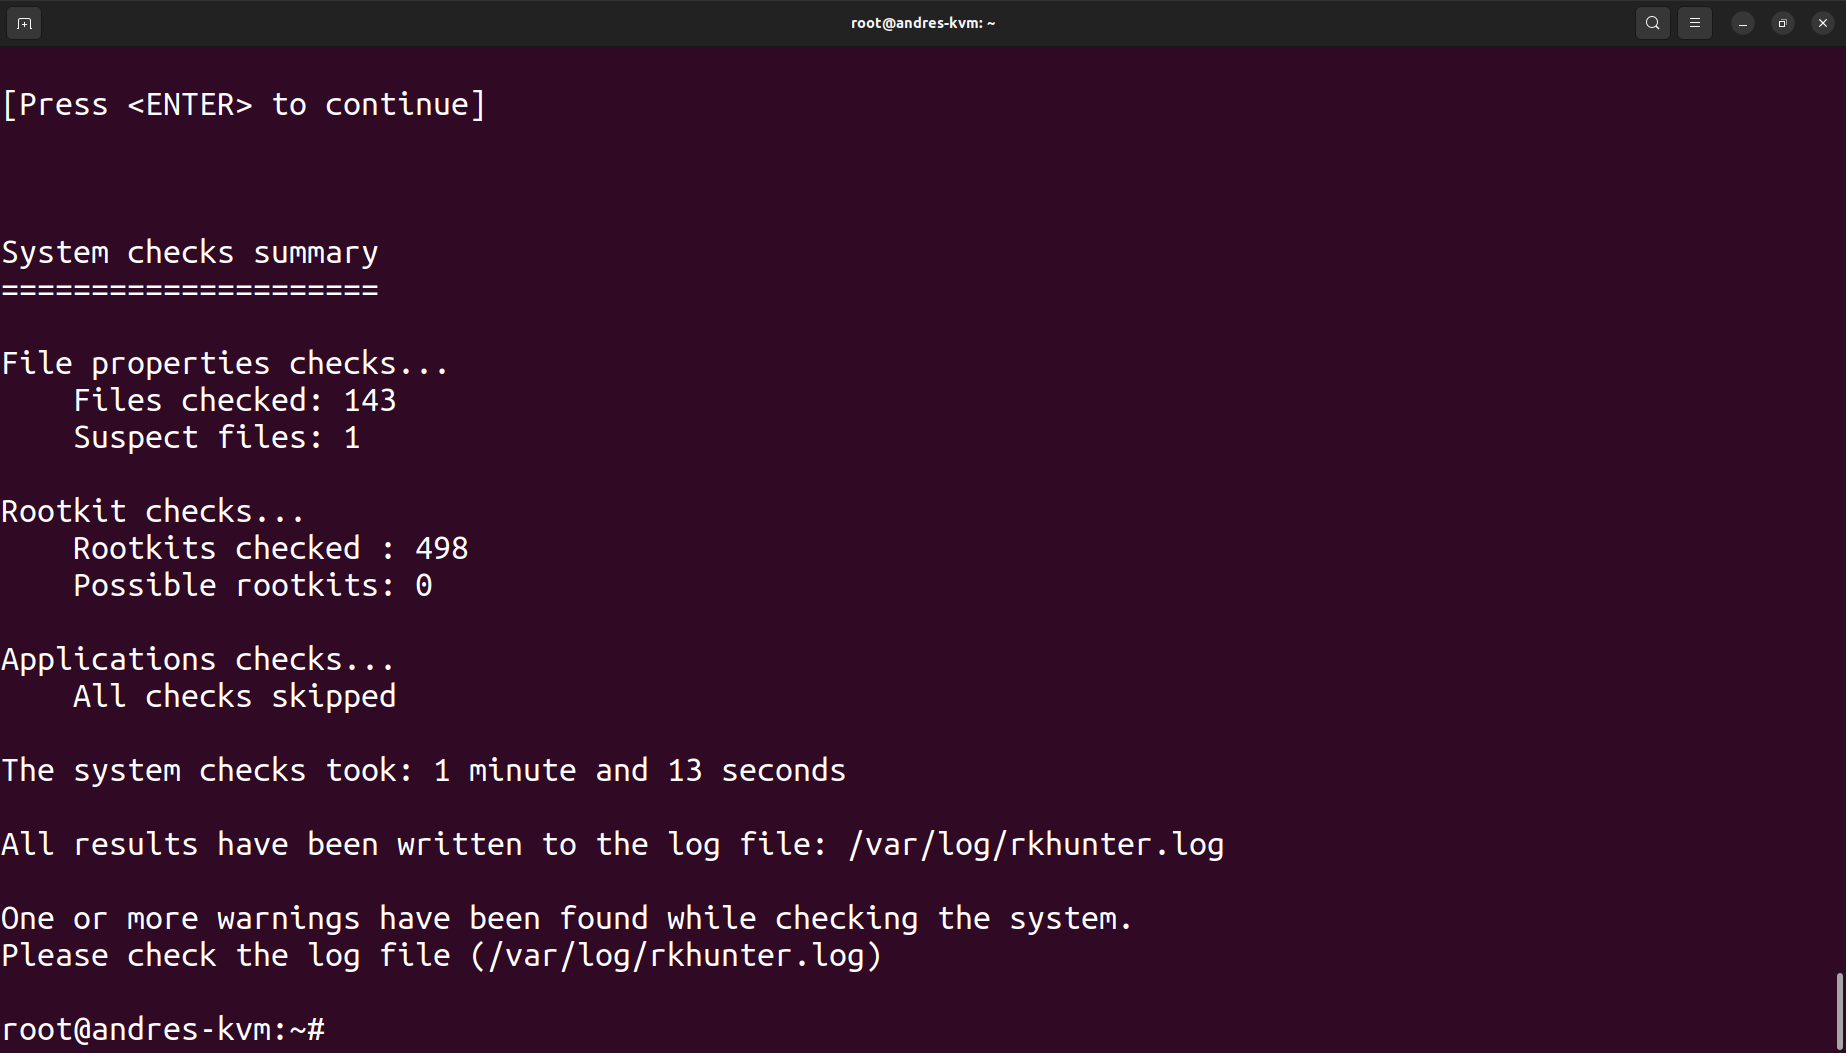
\includegraphics[width=\textwidth]{imagenes/rkhuntersalida1.png}
\end{figure}

Como se puede ver en los resultados, aparece que hay alguna advertencia. Ahora, revisando el archivo \verb|/var/log/rkhunter.log| y buscando la palabra ``Warning''.

\begin{figure}[H]
    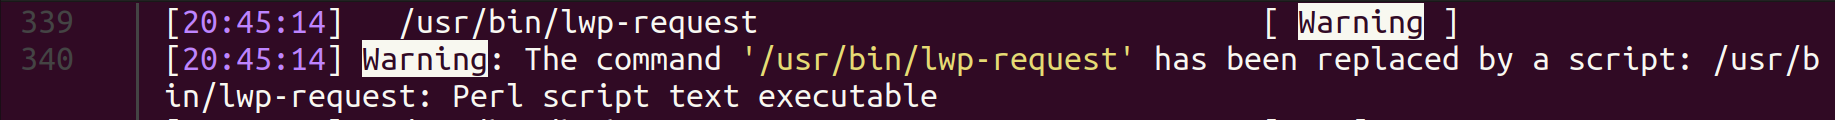
\includegraphics[width=\textwidth]{imagenes/warn1.png}
\end{figure}

La primera advertencia tiene que ver con la posible modificación del binario \verb|lwp-request|, en caso de ser una modificación malintencionada, un atacante podría modificar el binario para recibir todos los datos que se envían o reciben a través de él (por ejemplo, si se usa SSH, poner un keylogger para obtener las contraseñas).

\begin{figure}[H]
    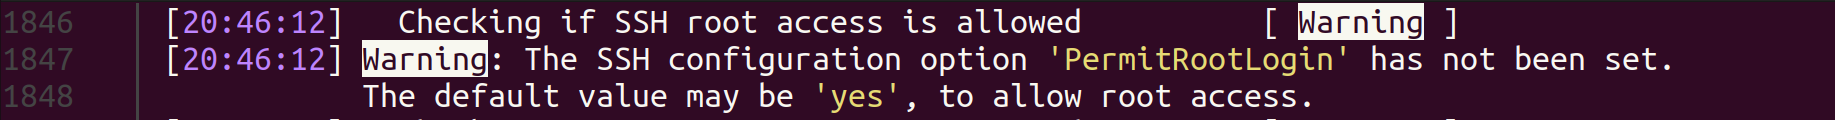
\includegraphics[width=\textwidth]{imagenes/warn2.png}
\end{figure}

\bigskip

La segunda advertencia tiene que ver con la seguridad de la configuración SSH, ya que el parámetro ``PermitRootLogin'' no está puesto a ningún valor y por defecto puede ser ``Yes'', dando la posibilidad de que un atacante pueda a entrar al sistema por SSH como usuario root.

\newpage

\addcontentsline{toc}{subsection}{Apartado B}
\subsection*{Apartado B}
El primer error se puede solucionar cambiando en \verb|/etc/rkhunter.log| el macro \verb|PKGMGR| (por defecto esta a ``NONE''), en el caso de Ubuntu y Debian se debe cambiar a ``DPKG''. Este cambio hace que coteje con los hashes de cada paquete para ver si han sido modificados malintencionadamente:

\begin{figure}[H]
    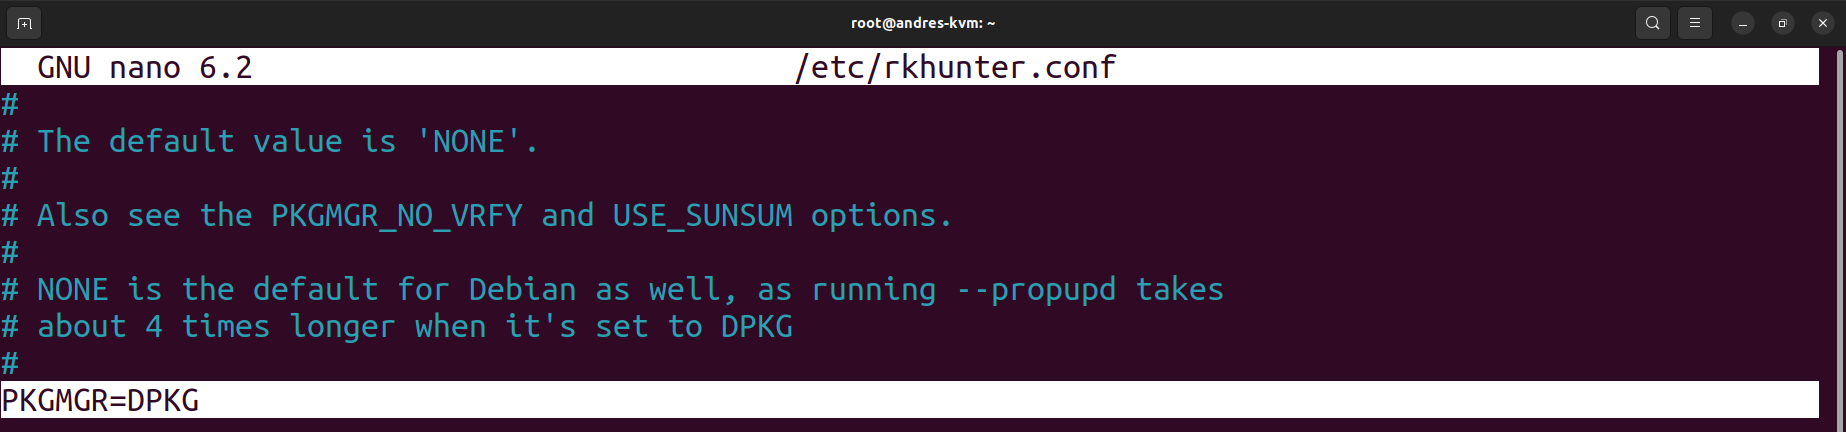
\includegraphics[width=\textwidth]{imagenes/rkhuntermacrodpkg.png}
\end{figure}

Una vez realizado este cambio, se debe ejecutar el comando \verb|sudo rkhunter --propupd|.


Todo esto se puede solucionar cambiando en el archivo de configuración \verb|/etc/ssh/sshd_config| y poniendo el parámetro a ``no'':

\begin{figure}[H]
    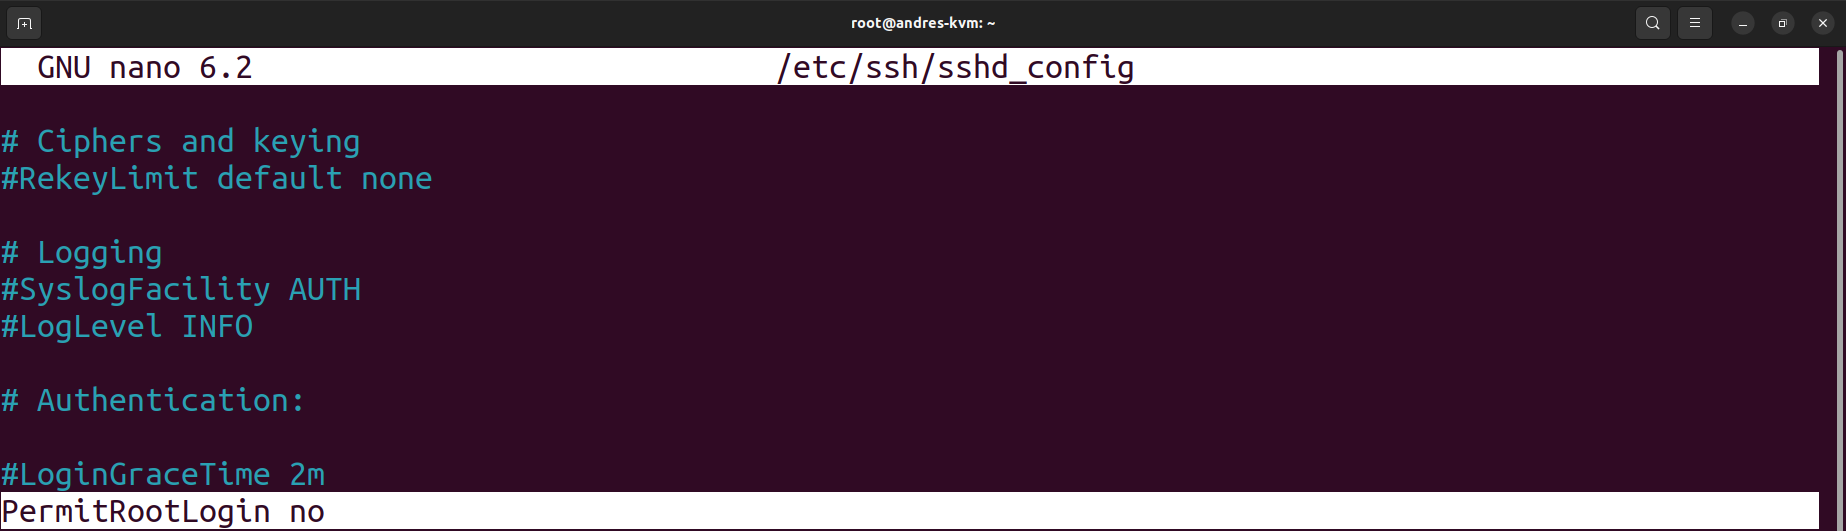
\includegraphics[width=\textwidth]{imagenes/sshpermit.png}
\end{figure}

Además, es necesario reiniciar el servicio con el comando \verb|systemctl restart ssh|.

Por último, para comprobar que el sistema ya no tiene más advertencias, ejecutamos de nuevo la orden \verb|sudo rkhunter --check|:

\begin{figure}[H]
    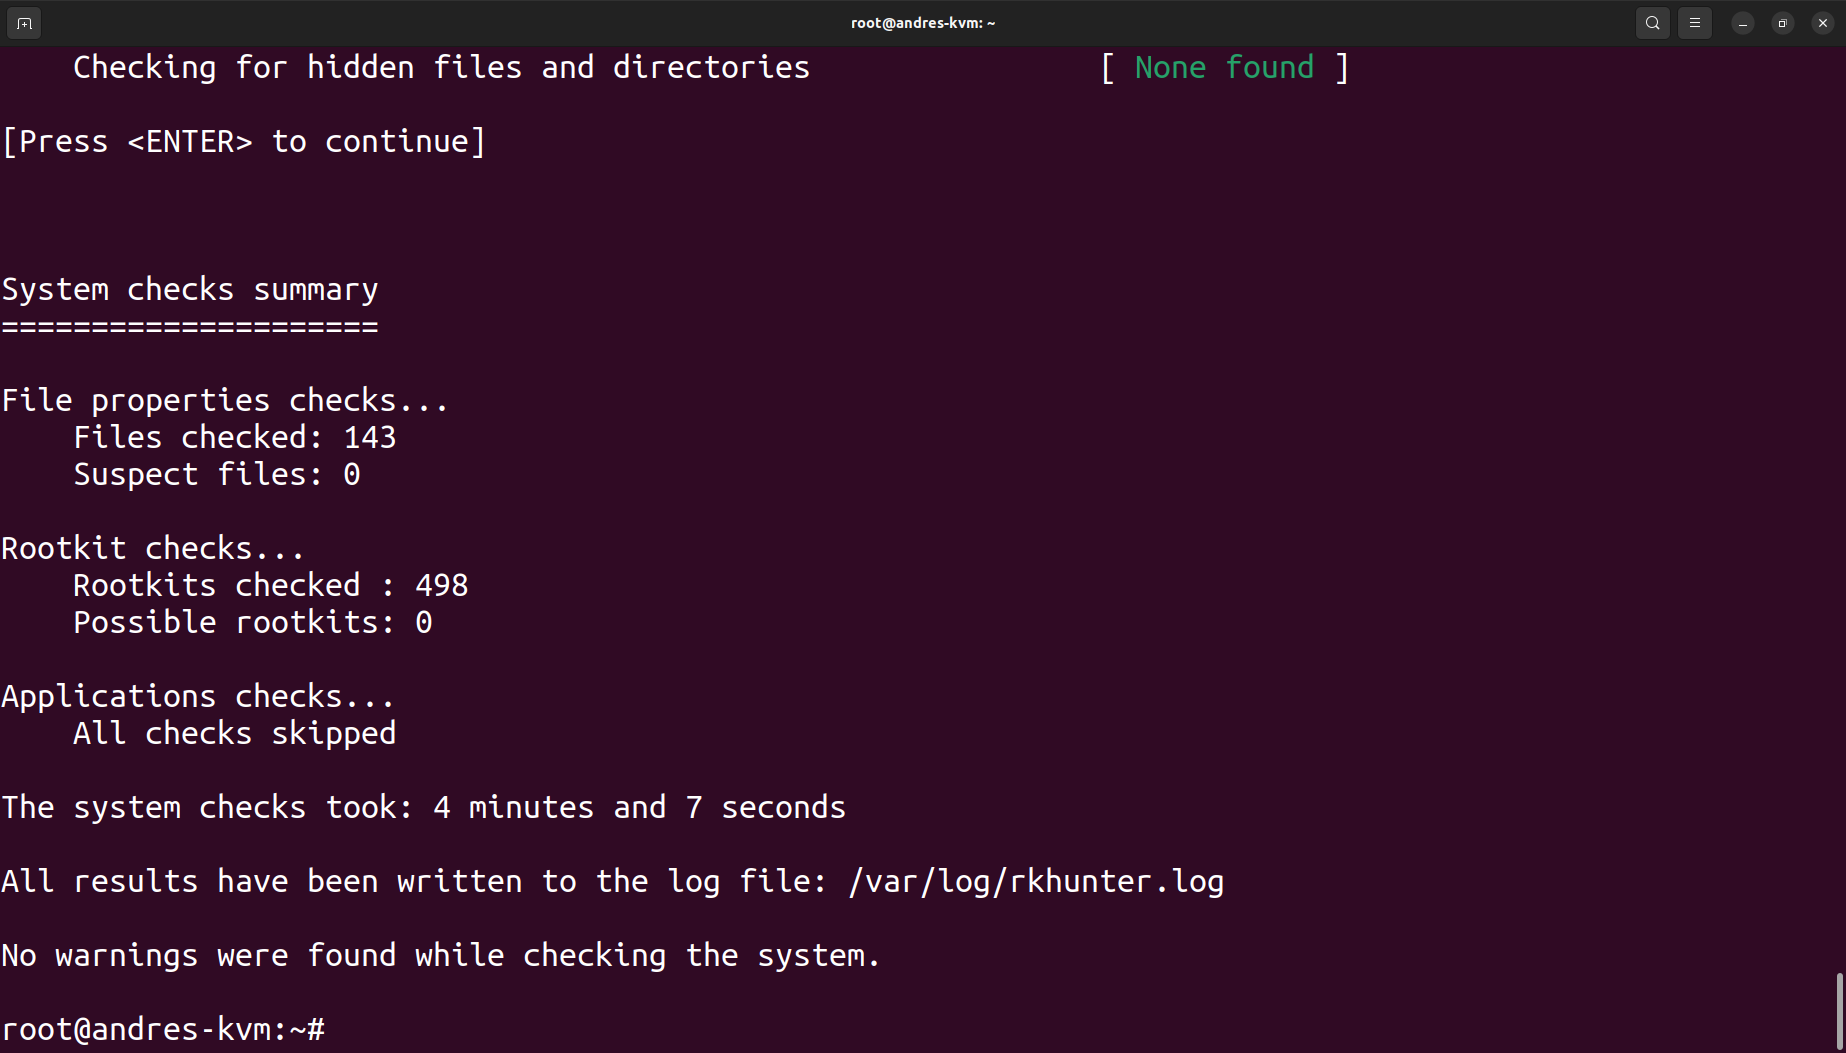
\includegraphics[width=\textwidth]{imagenes/rkhunterokk.png}
\end{figure}

Y como se puede ver, el sistema ya es seguro, eran solo falsos positivos en el primer caso, y en el segundo una mala configuración de un servicio importante.


\end{document}

%\begin{figure}[H]
%    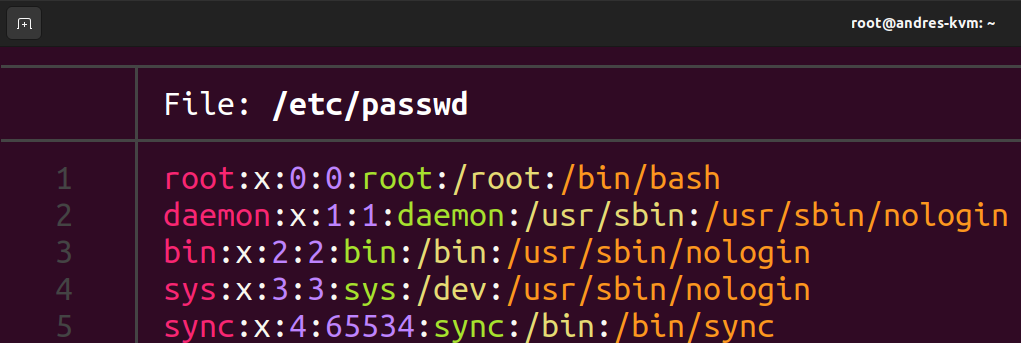
\includegraphics[width=\textwidth]{imagenes/passwdfile.png}
%    \caption{Ejemplo de entradas en el archivo.}
%\end{figure}